\documentclass[main.tex]{subfiles}
\setlength{\columnsep}{3cm}
\setcounter{secnumdepth}{3}
\begin{document}

\addtolength{\tabcolsep}{-2pt}

\section{Parallelizing Algorithms}
In the previous chapter, we discussed how \textit{Amdahl's Law} tells us how our programs are inherently bottlenecked by their non-parallelizable part, no matter how many processor we have available. Hence, it is our goal to reduce the sequential fraction of our programs when we want to run them on many processors. To this end, we introduce some methods to parallelize algorithms in this chapter, specifically in Java. Here, parallelization means that we divide up the task at hand onto different \textit{threads}, assuming that they are able to run on different \textit{processors}. This is in contrast to Chapter 3, where we assumed a fixed program that will be run on a single processor (imagine this is the work chunk a thread was assigned to process) and analyzed how we can exploit independence within this set of instructions.\\
We can use the techniques learned in this chapter to design parallel implementations of algorithms.

\subsection{Fork-Join Parallelism}
Let us once again consider the task of summing up an array. Using task parallelism, we can simply divide up the array on some number of threads. Each thread sums up some part of the array and finally, the main thread sums up these partial results. The corresponding code looks something like this in Java:
\begin{figure}[H]
    \begin{minted}[]{java}
int sum(int[] arr) { // can be a static method
    int len = arr.length;
    int ans = 0;
    SumThread[] ts = new SumThread[4];
    for (int i = 0; i < 4; i++) { // do parallel computations
        ts[i] = new SumThread(arr, i*len/4, (i+1)*len/4);
        ts[i].start();
    }
    for (int i=0; i < 4; i++) { // combine results
        ts[i].join(); // wait for helper to finish!
        ans += ts[i].ans;
    }
    return ans;
}
    \end{minted}
\end{figure}
\noindent Here, \texttt{SumThread} is some \texttt{Thread} class summing up the given indices. We do not really care about its exact implementation here.\\[3mm]
This approach of dividing up the work into multiple different tasks and then combining their results is called \textit{Fork-Join Parallelism}. The join in fork/join does not necessarily refer to the \texttt{Thread.join()} method, where we wait for a thread to finish, but can also mean the combination of the partial results (in this case the main threads sums up the partial results).

\subsubsection{Parallel Divide-And-Conquer}
Above solution is not new to us. But we will improve upon it. Assume we want to run above code on some hardware efficiently. We find a few things that are not optimal with this general approach:
\begin{itemize}
  \item There is a fixed number of threads created (four in this case), no matter how many processors the underlying hardware has. We can solve this by making the number of threads created a parameter of the method.
  \item For general datastructures, dividing it into equal chunks for threads to process can lead to large workload imbalances across threads. Consider a graph datastructure. When we give the same number of vertices to each thread to process, the number of edges in a vertex set might be vastly different. When we now want to run parallel BFS, we will not get good speedup, because the few threads with the most edges will bottleneck the runtime. In this case, this is not a problem, since each thread will have about the same workload with summing array entries.
  \item We have a sequential bottleneck of summing up the partial results in the end.
\end{itemize}
We can improve on the last point by parallelizing the result combination. This can easily be implemented by recursively dividing the tasks with the Fork-Join model. This gives us a parallel version of the \textit{divide-and-conquer} paradigm. The basic structure of a divide-and-conquer program is the following:

\begin{figure}[H]
    \centering
    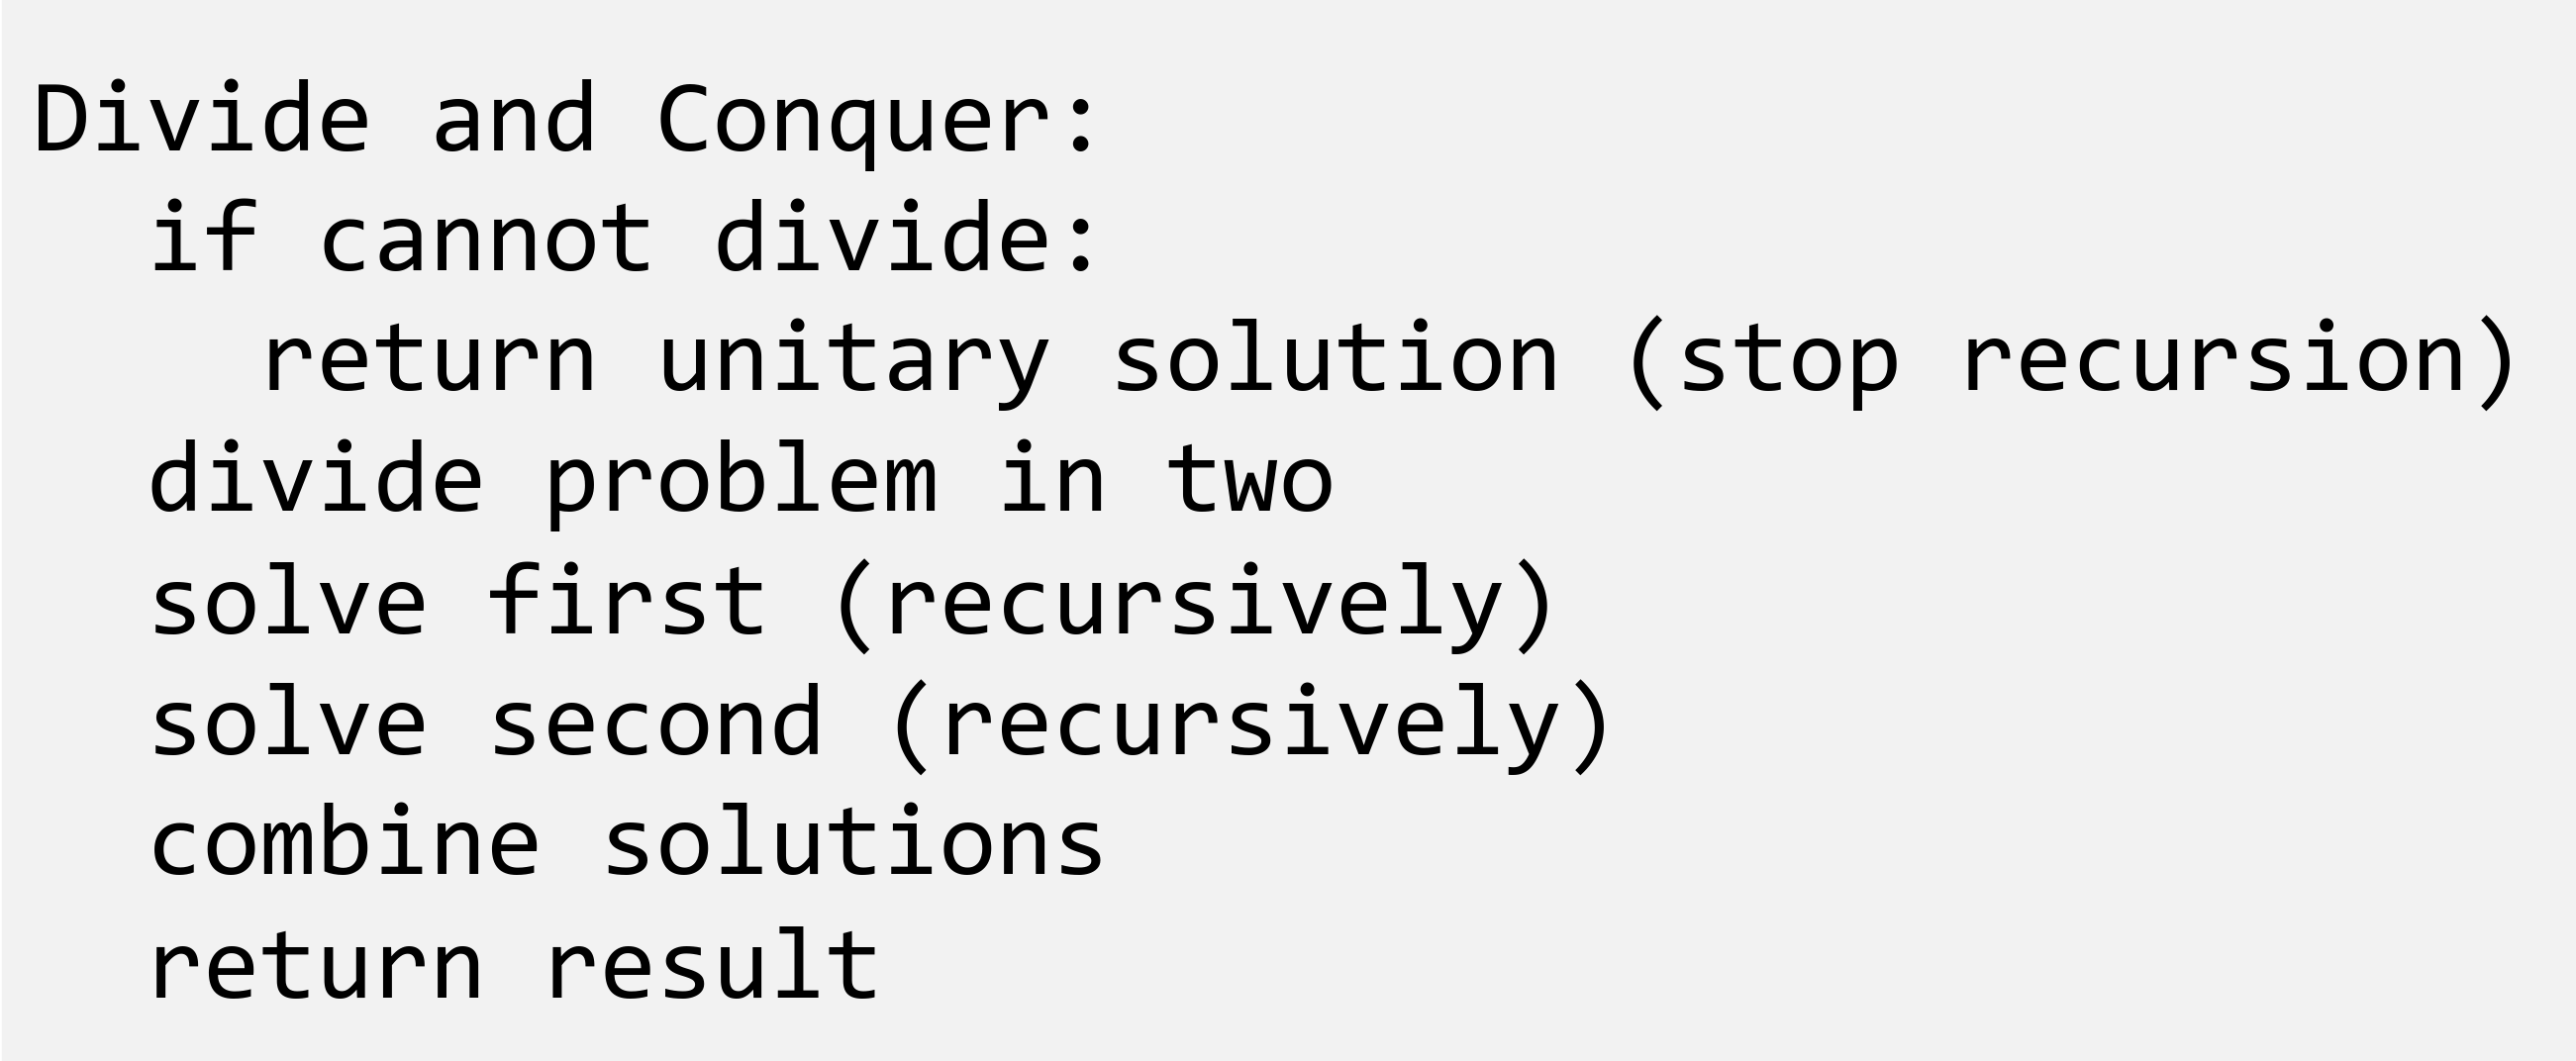
\includegraphics[scale=0.08]{DivideAndConquer.png}
    \caption{Structure of a Divide-and-Conquer Program.}
\end{figure}

\noindent We can implement this with the following code:
\begin{minted}[]{java}
public static int do_sum_rec(int[] arr, int startIdx, int endIdx) {
    int size = endIdx-startIdx;
    if (size == 1) // check for termination criteria
        return arr[startIdx];
    // split array in half and call self recursively
    int mid = size / 2;
    int sum1 = do_sum_rec(arr, startIdx, startIdx + mid);
    int sum2 = do_sum_rec(arr, startIdx + mid, endIdx);
    return sum1 + sum2;
}
\end{minted}
\noindent We can trivially parallelize this by solving the recursion for the first and second subproblem in parallel. We get the following structure of function calls:
\begin{figure}[H]
    \centering
    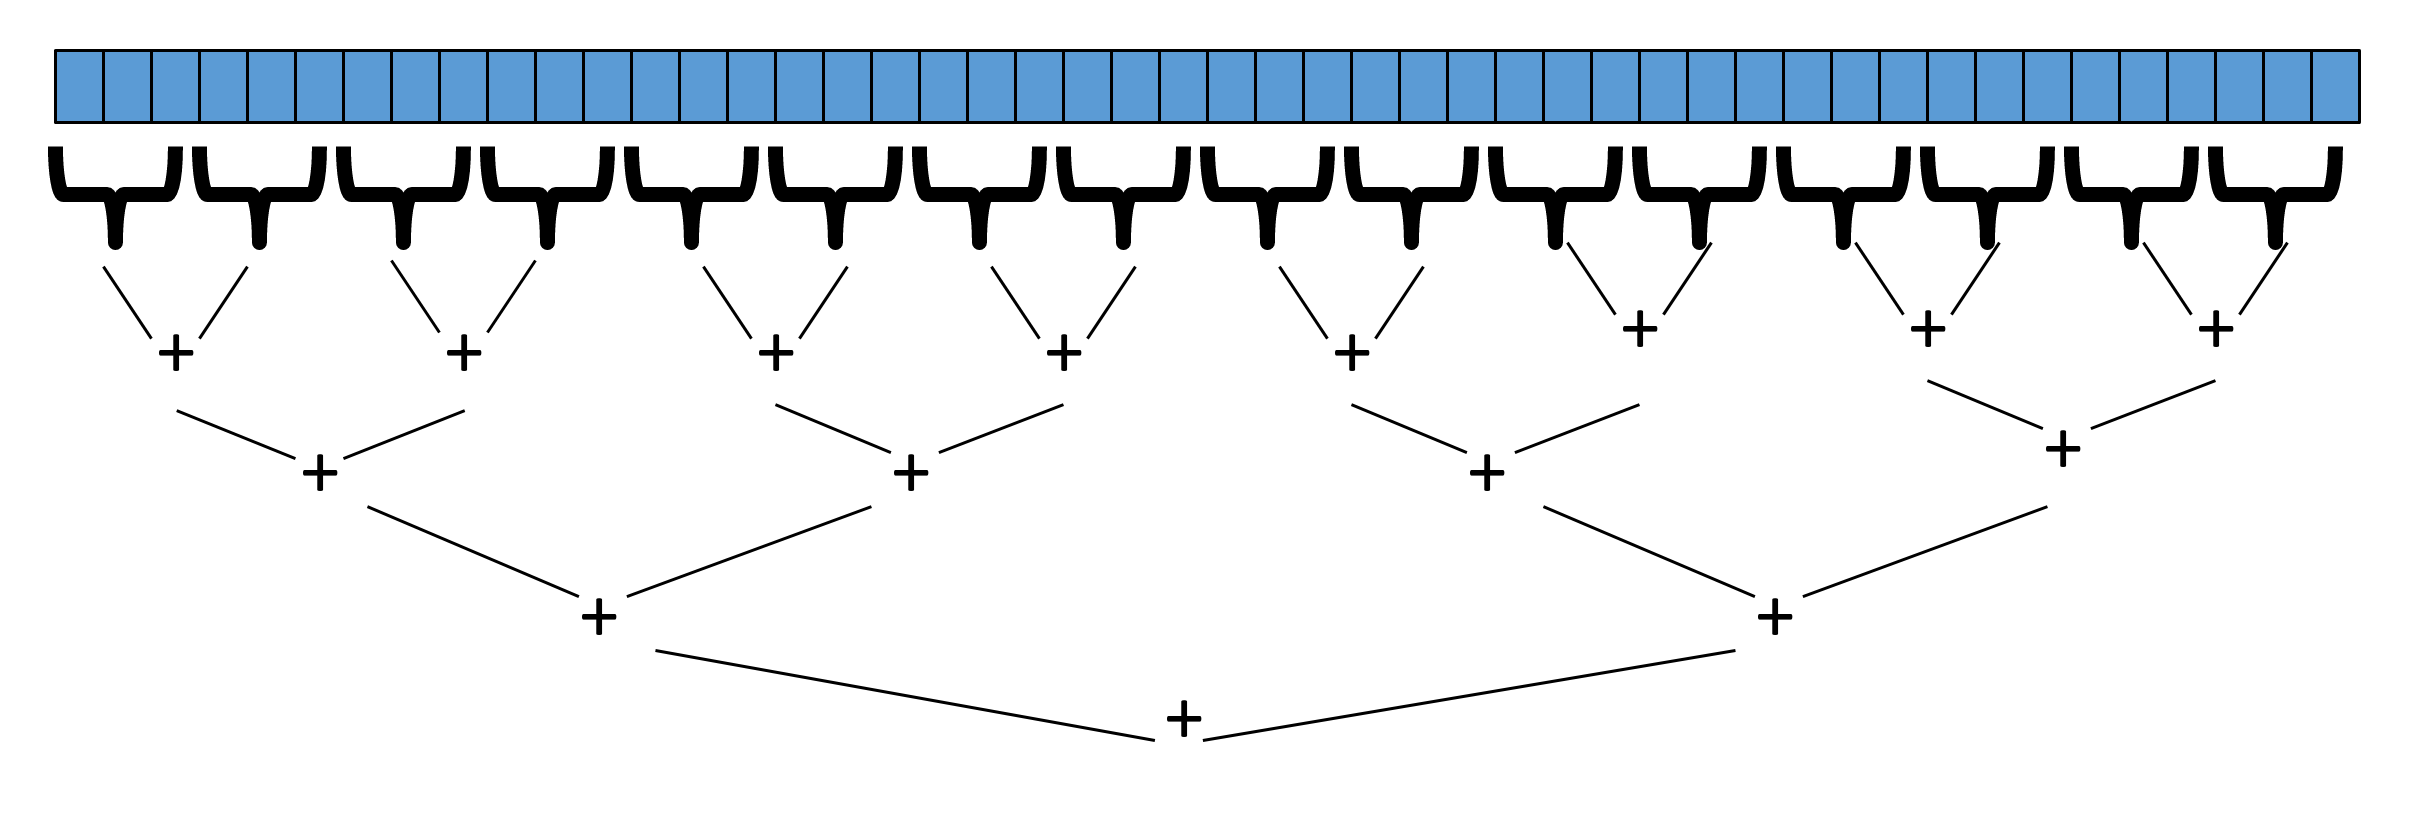
\includegraphics[scale=0.15]{DnCTree.png}
    \caption{Structure of a Divide-and-Conquer Program.}
\end{figure}
\noindent Function calls on the same level in the tree can be executed in parallel. Notice that the tree has a depth logarithmic in the number of array entries. This is much better than what we can achieve by simply dividing up the array between threads.\\
Although to actually get the logarithmic runtime, we require as many processors as array entries. Else, the threads on the last level cannot all run in parallel.  But this approach is still superior compared to our initial approach with dividing the array into equal chunks, because it solves two previously mentioned problems:
\begin{itemize}
  \item The sequential bottleneck of summing up the partial results is resolved since even the result combination is parallelized, allowing for more speedup with increasing number of processors.
  \item It is easier to implement more equal load balancing. Consider again a graph as an input datastructure. When a task divides up its assigned vertices on two subtasks, it can also count the number of edges in the two sets and adjust the division accordingly (such that both subtasks get not just a similar amount of vertices, but also a similar amount of edges). This is a much simpler problem than when we have to partition the entire graph on \textit{n} threads in the beginning.
\end{itemize}

\newpage

\subsubsection{Parallel Divide-And-Conquer with Java Threads}
But now, how do we implement this parallelization of the two subtasks? Of course we can create two threads solving each half recursively. This would look something like this:
\begin{minted}[]{java}
public void run() {
    int size = endIdx - startIdx;
    if (size == 1) {
        result = arr[startIdx];
        return;
    }
    int mid = size / 2;
    SumThread t1 = new SumThread(arr, startIdx, startIdx + mid);
    SumThread t2 = new SumThread(arr, startIdx + mid, endIdx);
    t1.start();
    t2.start();
    t1.join(); // join() would have to be in a try-catch block
    t2.join();
    result = t1.result + t2.result;
    return;
}
\end{minted}
\noindent Now imagine we want to process arbitrarily large arrays like this. Remember that each Java thread is mapped to an OS thread. Also remember that each OS thread gets some resources, for example a stack. This is a small region of memory residing in main memory. When we now create millions of threads for a large array, we will sooner or later run out of memory. This will be visible with the following error:

\begin{figure}[H]
    \centering
    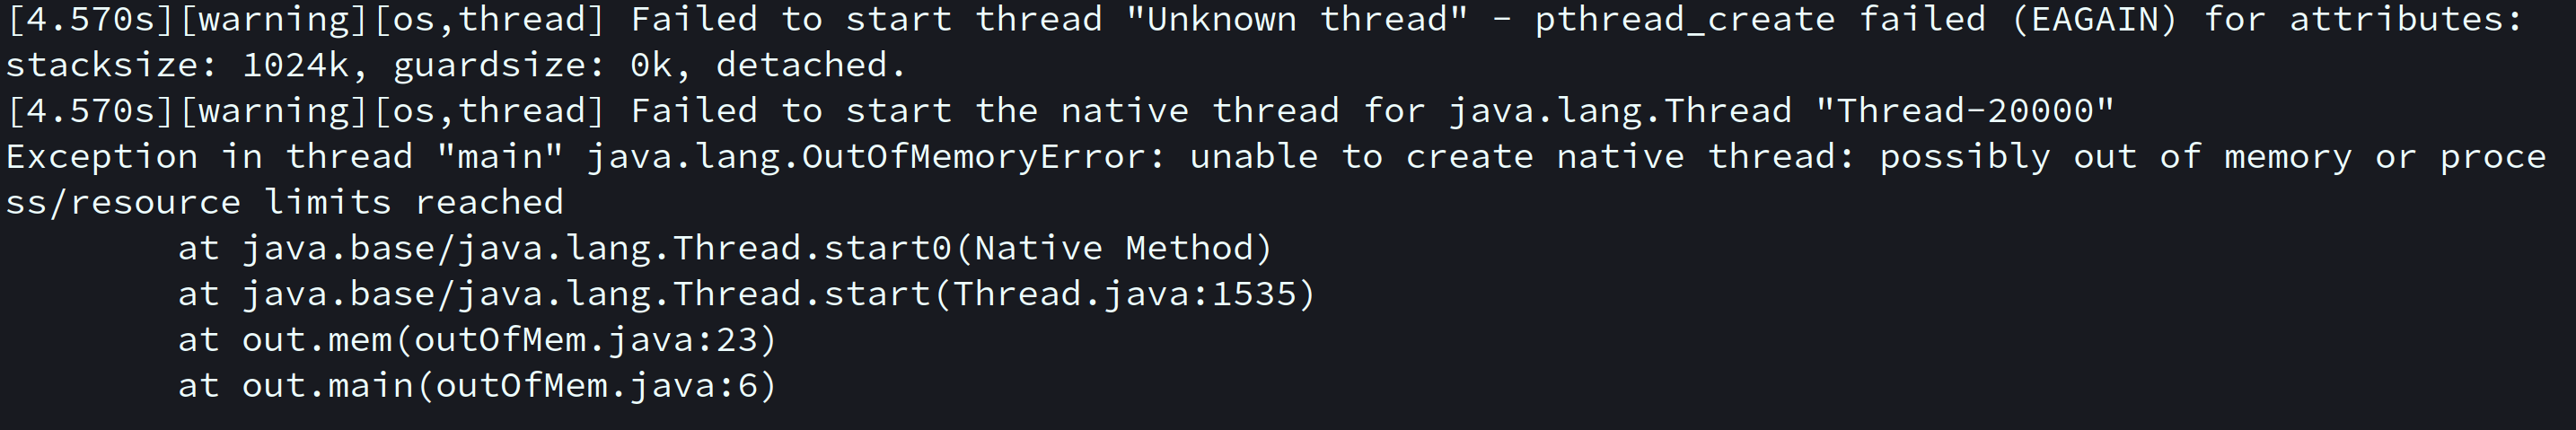
\includegraphics[scale=0.15]{OutOfMem.png}
    \caption{OutOfMemoryError-Exception due to creating too many threads in Java.}
\end{figure}

\noindent Implementing parallel divide-and-conquer with native Java threads is not feasible due to their resource consumption. Using native Java threads for recursive subtasks is not suitable for a number of reasons anyways:

\begin{itemize}
  \item \textbf{Resource blocking:} A thread will join the new threads it creates and potentially wait for a long time for them to return. In this time, the Java Thread object blocks an OS thread, which may be idle (does not use up CPU time, which is good), but still blocks the resources allocated for it. When we have millions of threads, most of which are currently joining, large chunks of memory are allocated, even though few threads are doing actual work.
  \item \textbf{Many more threads than cores:} We probably do not have millions of cores to run the code on. Therefore, we cannot possibly gain an advantage by creating so many (Java and thus OS) threads. Remember that creating OS threads brings some overhead. Also, context switching between the threads is expensive, so we never want to have many more active OS threads than we have processors.
\end{itemize}

\noindent The problem we have is fundamentally that Java threads are too \textit{heavy-weight} for these recursive tasks. The recursive tasks do not each require their own OS thread, which is what is given to them when we create Java threads.\\
Remember that in chapter 1, we said that many languages have something like virtual threads. That is, the user creates virtual threads (or tasks) and the language runtime decides itself how these are going to be mapped to OS threads. The advantage is that by using this approach, the virtual threads are (potentially) much less heavy-weight than when simply one-to-one mapping to OS threads, solving all of our problems.

\subsubsection{Manually Optimizing Divide-And-Conquer using Java Threads}
Before we look into solutions to this problem of Java threads being too heavy-weight, let us perform two manual optimizations:

\begin{enumerate}
  \item Currently, we break down the problem until the assigned chunk size equals one. This is not efficient, as thread creation brings some overhead. Say we process a chunk of 20 array elements. When we divide this onto two new threads, each only has to process 10 elements. However, the time required to create and start new threads is significantly longer than the time gained to process 10 instead of 20 elements. Hence, we introduce a \textbf{cutoff} at, say, 1000 elements. As soon as the assigned array chunk has length less than 1000, the thread will sum it itself and not divide it any further. Using this optimization, we need to create fewer threads.
  \item When we create two threads to solve each half of the problem, the thread creating them has nothing to do while waiting on the two results but still blocks resources. It would be more efficient when the thread solves one half itself and outsources the second half to another thread to solve concurrently. We can do this by calling \texttt{Thread.run()} instead of \texttt{Thread.start()}. This again means that we need to create fewer threads.
\end{enumerate}

\noindent Using these two optimizations, we receive the following code:

\begin{minted}[]{java}
public void run() {
    int size = endIdx - startIdx;
    if (size <= 1000) {
        result = 0;
        for (int i = startIdx; i < endIdx; i++) {
            result += arr[i];
        }
        return;
    }
    int mid = size / 2;
    SumThread t1 = new SumThread(arr, startIdx, startIdx + mid);
    SumThread t2 = new SumThread(arr, startIdx + mid, endIdx);
    t1.start();
    t2.run(); // executes the run() method of t2 with the current thread
    t1.join(); // join() would have to be in a try-catch block
    result = t1.result + t2.result;
    return;
}
\end{minted}

\noindent Even with these optimizations, our problem with Java threads being too heavy-weight remains due to resource-blocking, creation and context switching overhead. These optimizations simply mean that we create less threads overall, but for sufficiently large arrays, the exact same problems occur.

\subsubsection{Solving Heavy-Weight Threads in Java: ExecutorService}
\label{ExecutorService}
Java provides us the \texttt{ExecutorService} framework as an abstraction layer between tasks and threads. Instead of creating a thread to solve one half of the array recursively, we create a \textit{task} and submit it to an \texttt{ExecutorService}. The \texttt{ExecutorService} then maps these tasks to Java threads itself. This scheduling of tasks to Java threads is similar to what the OS does on a lower abstraction level, where it maps OS threads to available processors.\\[3mm]
This seems to be exactly what we need to solve our issue with the heavy-weight Java threads. Let us create an \texttt{ExecutorService} instance in Java:
\begin{minted}[]{java}
// Create an ExecutorService with a fixed thread pool of 4 threads
ExecutorService executor = Executors.newFixedThreadPool(4);
\end{minted}
\noindent Here, we give the \texttt{ExecutorService} instance a pool of four threads. This means that the service will create four threads when initialized. When we now submit tasks, these will wait in a queue for a thread in the pool to become available.
\begin{figure}[H]
    \centering
    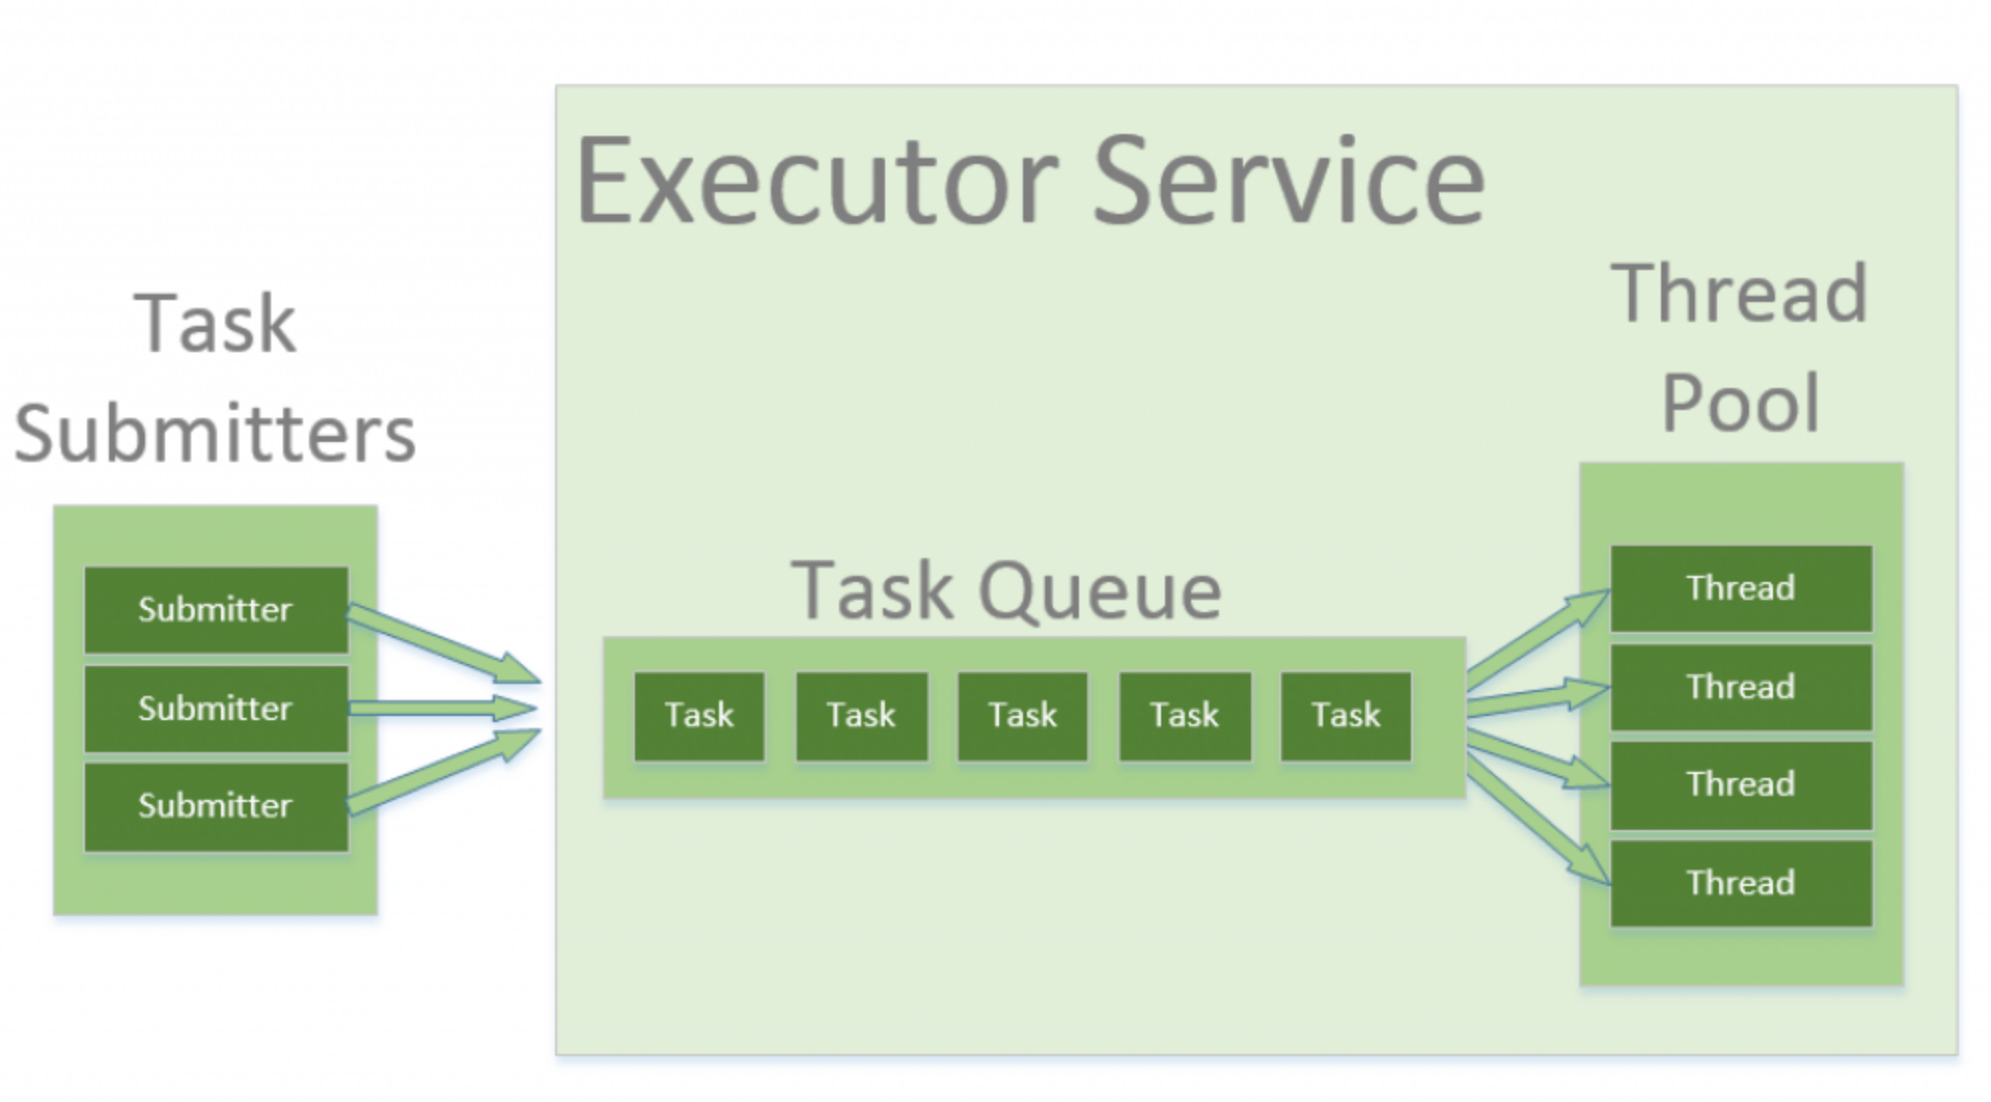
\includegraphics[scale=0.13]{ExecutorServiceQueue.png}
    \caption{Internal structure of \texttt{ExecutorService} with a fixed thread pool: https://www.baeldung.com/thread-pool-java-and-guava}
\end{figure}
\noindent What exactly do we submit to the \texttt{ExecutorService} now? Threads? Almost. Remember that we could create a Java Thread object by initializing it with a \texttt{Runnable} object? We can submit exactly such \texttt{Runnable} objects to the \texttt{ExecutorService} (and also others). Some important methods of \texttt{ExecutorService} are the following. Let \textit{ex} be an \texttt{ExecutorService} instance in our code.
\begin{itemize}
  \item \texttt{ex.submit(Runnable task)}: Submits a Runnable object for execution and returns a Future object representing that task.
  \item \texttt{ex.submit(Callable<T> task)}: Submits a value-returning task for execution and returns a Future object representing the pending results of the task. This allows us to submit a \texttt{Callable<T>} object (think of a Runnable object that can return a value of type T and implements the \texttt{call()} function instead of the \texttt{run()} function).
  \item \texttt{ex.shutdown()}: Initiates an orderly shutdown in which previously submitted tasks are executed, but no new tasks will be accepted. After all previously submitted tasks are executed, the thread pool is deallocated. We always call this method when we finish using the \texttt{ExecutorService} instance.
\end{itemize}
\noindent When we submit tasks, \texttt{ExecutorService} returns us a Future object. This provides us a handle for the submitted task to for example request the result or check its progress. Let us write a simple program using \texttt{ExecutorService} to get a better idea of what we can do.

\begin{minted}[]{java}
public static void main(String[] args) {
    /* submit 100 callables to the service and store the returned
     Future objects in a list */
    ExecutorService ex = Executors.newFixedThreadPool(4);
    List<Future<Integer>> futures = new ArrayList<>();
    for (int i = 0; i < 100; i++) {
        Future<Integer> future = ex.submit(new MyCallable());
        futures.add(future);
    }

    // sum up the results of all tasks
    int sum = 0;
    for (Future<Integer> future : futures) {
        try {
            sum += future.get();
        } catch (InterruptedException | ExecutionException e) {
            e.printStackTrace();
        }
    }

    System.out.println("Sum of all results: " + sum);
    ex.shutdown();
}
\end{minted}

\newpage

\begin{minted}[]{java}
class MyCallable implements Callable<Integer> {
    /* implement the call() method. The call() method is the code the task
     executes when it is its turn */
    public Integer call() throws Exception {
        int sum = 0;
        for (int i = 0; i < 10; i++) {
            sum += i;
        }
        return sum;
    }
}
\end{minted}

\noindent We can see that when calling \texttt{future.get()}, we get the result of the computation. When using threads, we first need to call \texttt{thread.join()} to ensure the computation is completed. But here, the underlying threads are abstracted away and calling \texttt{future.get()} automatically waits on the task being finished, without having to join.

\subsubsubsection{Parallel Divide-And-Conquer with \texttt{ExecutorService}}
With \texttt{ExecutorService}, we can now try implementing our parallel divide-and-conquer program again. Since we can create a fixed thread pool, we will not have the same issue of running out of memory, no matter the array size. Let us implement the \texttt{call()} method of a corresponding \texttt{Callable} class using \texttt{ExecutorService}:
\begin{minted}[]{java}
public class SumRecCall implements Callable {
    ...

    public Integer call() throws Exception {
        int size = endIdx - startIdx;
        if (size <= 1000) {
            int result = 0;
            for (int i = startIdx; i < endIdx; i++) {
                result += arr[i];
            }
            return result;
        }
        int mid = size / 2;
        SumRecCall c1 = new SumRecCall(ex, arr, startIdx, startIdx + mid);
        SumRecCall c2 = new SumRecCall(ex, arr, startIdx + mid, endIdx);
        Future<Integer> f1 = ex.submit(c1);
        Future<Integer> f2 = ex.submit(c2);
        return f1.get() + f2.get();
    }

    ...

}
\end{minted}

\begin{minted}[]{java}
// main method defined somewhere else
public static void main(String[] args) {
    ExecutorService ex = Executors.newFixedThreadPool(4);
    SumRecCall task = new SumRecCall(ex, arr, 0, arr.length);
    Future<Integer> result = ex.submit(task);
    System.out.println(result.get());
    ex.shutdown();
}
\end{minted}
\noindent When we now run this program, we notice that it does not return. To understand what happens, let us consider the workings of \texttt{ExecutorService} again. A submitted task is put in a wait queue, where it waits until one of the four threads in the pool is free. Now, let us consider what happens with the first five tasks submitted in this code:
\begin{itemize}
  \item The first task gets the whole array to process, hence it creates and submits two further tasks to process each half. However, this first task is assigned to the first thread in the pool. It will keep occupying this thread, even when it now has to wait for its subtasks to complete.
  \item The two tasks created by the first task occupy the second and third thread in the pool, meaning only one thread remains free. Since the array is presumably quite long, these two tasks will again create two more tasks each (to solve each of their problem half) and submit them to the service. Again, even though they are waiting for a Future to return its result, they all occupy a thread in the pool and will not let it go until they completed their \texttt{call()} method.
  \item Task four will get the last thread in the pool. The fifth task that is submitted will not find a free thread in the pool anymore. That means that it will wait in the queue for a thread to become free. However, this will not happen, as the tasks currently occupying the thread are waiting for the tasks in the queue to return their result. They of course cannot do this without a thread. We have reached a deadlock.
\end{itemize}
This seems very disappointing at first. The fixed thread pool of the executor service is not made for tasks that create further tasks themselves. An example for a useful application using the fixed thread pool of \texttt{ExecutorService} is handling HTTP requests of a webserver. Each request is submitted to the \texttt{ExecutorService} as a task and the service distributes the tasks across the available threads.

\subsubsection{Java Fork/Join Framework}
When we browse the Java documentation, we find that \texttt{ExecutorService} is an interface. Remember that interfaces in Java define some high-level behaviour by declaring methods that classes can then specifically implement. We can instantiate an \texttt{ExecutorService} for example through the fixed thread pool we saw earlier. There is another interesting implementation of the \texttt{ExecutorService} interface called \texttt{ForkJoinPool}. This class is the center of Java's fork/join framework and designed for recursive tasks, exactly what we are looking for. We can instantiate a \texttt{ForkJoinPool} in the following way:

\begin{minted}[]{java}
ForkJoinPool fj = new ForkJoinPool(4);
fj.invoke(new Task());
fj.shutdown();
\end{minted}

\noindent Assuming that the class \texttt{Task} is some kind of generic task the \texttt{ForkJoinPool} accepts, this code creates a \texttt{ForkJoinPool} that uses a maximum of four Java threads and starts a \texttt{Task} object. With our previous knowledge, we can characterize the \texttt{ForkJoinPool} class with a few points:

\begin{itemize}
  \item A \texttt{ForkJoinPool} is an implementation of the \texttt{ExecutorService} interface. We can instantiate it (among other possibilities) by specifying the maximum number of used Java threads as an argument. When we do not give any argument, the thread pool will by default contain as many threads as there are cores available on the system.
  \item The difference to the \texttt{ExecutorService} thread pools we previously saw is that it employs \textbf{work stealing}. We will elaborate on this, but in a nutshell, it means that instead of simply waiting for subtasks to finish, threads in the fork/join Framework steal tasks from other threads to execute in the meantime. This is the key feature that prevents the deadlock problem we previously had with \texttt{ExecutorService}.
  \item The tasks that a \texttt{ForkJoinPool} accepts are \texttt{ForkJoinTask}s. The \texttt{ForkJoinTask} class is an abstract base class, with the relevant subclasses being \texttt{RecursiveTask<V>} and \texttt{RecursiveAction} (similar to \texttt{Callable<T>} and \texttt{Runnable}). So, we invoke our \texttt{ForkJoinPool} usually with either a \texttt{RecursiveTask<V>} (when we require our tasks to return a value of type V) or a \texttt{RecursiveAction} object (if no return value is required).
  \item To start subtasks from within a task, we can call \texttt{ForkJoinTask.fork()} and then \texttt{ForkJoinTask.join()} to wait for the computation to be finished.
\end{itemize}

\subsubsubsection{Parallel Divide-And-Conquer with Fork/Join Framework}
\noindent Let us now finally implement our parallel array sum algorithm using the fork/join framework:

\begin{minted}[]{java}
public int sumArray(int[] arr) {
    ForkJoinPool fj = new ForkJoinPool(4);
    SumRecCall sumTask = new SumRecCall(arr, 0, arr.length);
    int result = fj.invoke(sumTask);
    fj.shutdown();
    return result;
}
\end{minted}

\begin{minted}[]{java}
class SumRecCall extends RecursiveTask<Integer> {
    int[] arr;
    int endIdx, startIdx;

    // constructor
    public SumRecCall(int[] arr, int startIdx, int endIdx) {
        this.arr = arr;
        this.startIdx = startIdx;
        this.endIdx = endIdx;
    }

    public Integer compute() {
        int size = endIdx - startIdx;
        if (size <= 1000) {
            int result = 0;
            for (int i = startIdx; i < endIdx; i++) {
                result += arr[i];
            }
            return result;
        }
        int mid = size / 2;
        SumRecCall first = new SumRecCall(arr, startIdx, startIdx + mid);
        SumRecCall second = new SumRecCall(arr, startIdx + mid, endIdx);
        first.fork();
        second.fork();
        int firstSum = first.join();
        int secondSum = second.join();
        return firstSum + secondSum;
    }
}
\end{minted}

\noindent We see that the syntax is similar to our previous approach using a fixed thread pool for an \texttt{ExecutorService}. Differently though, we do not need to store a \texttt{Future} object returned by the task. This is because the \texttt{RecursiveTask} \textit{is} the \texttt{Future} object (the \texttt{RecursiveTask} and \texttt{RecursiveAction} classes implement the \texttt{Future} interface). Hence, we can simply get the result by calling \texttt{ForkJoinTask.join()}.\\[3mm]
Note that we could compute one half on the current thread by calling \texttt{second.compute()} instead of \texttt{second.fork()} to perform the same manual optimization as we did when using Java threads. However, this provides us no advantage in the fork/join framework as the task scheduler of the framework optimizes this by itself. So, we can neatly \texttt{fork()} and \texttt{join()} both tasks and need not worry about performance.\\
However, the optimization to set a sequential cutoff is still important to make sure each task provides enough work. This is because while we do not create a new thread for each task anymore, there is still some overhead to enqueue this task and schedule it on the worker threads in the pool. Setting the threshold to something like 1000 array elements is reasonable in this case to strike a good balance between exploiting parallelism and ensuring the task creation overhead does not dominate execution time.

\subsubsubsection{Work-Stealing in the Fork/Join Framework}
We mentioned that the fork/join framework solves the deadlock problem other \texttt{ExecutorService} implementations have by means of employing a work-stealing algorithm for scheduling submitted tasks among threads in the pool.\\[3mm]
Remember from \ref{ExecutorService} (\texttt{ExecutorService} introduction) that the submitted tasks within an \texttt{ExecutorService} enter a queue where they wait for a free thread in the pool. The fork/join framework now implements work-stealing in the following way:

\begin{itemize}
  \item Each thread in the \texttt{ForkJoinPool} additionally maintains its own double-ended queue of assigned tasks.
  \item When a thread in the pool runs out of tasks (i.e. its queue becomes empty), it attempts to \textit{steal} tasks from the queues of other threads in the pool.
  \item When a thread in the pool encounters a \texttt{ForkJoinTask.join()} operation (meaning it has to wait for the result/termination of the computation) it processes other tasks from the queue until the joined task is finished.
\end{itemize}

\noindent With this additonal queue per thread and the threads processing other tasks upon a \texttt{join()} operation, the recursion required by parallel divide-and-conquer is finally possible in an efficient manner. We can visualize the workings of the fork/join framework in the following way:


\begin{figure}[H]
    \centering
    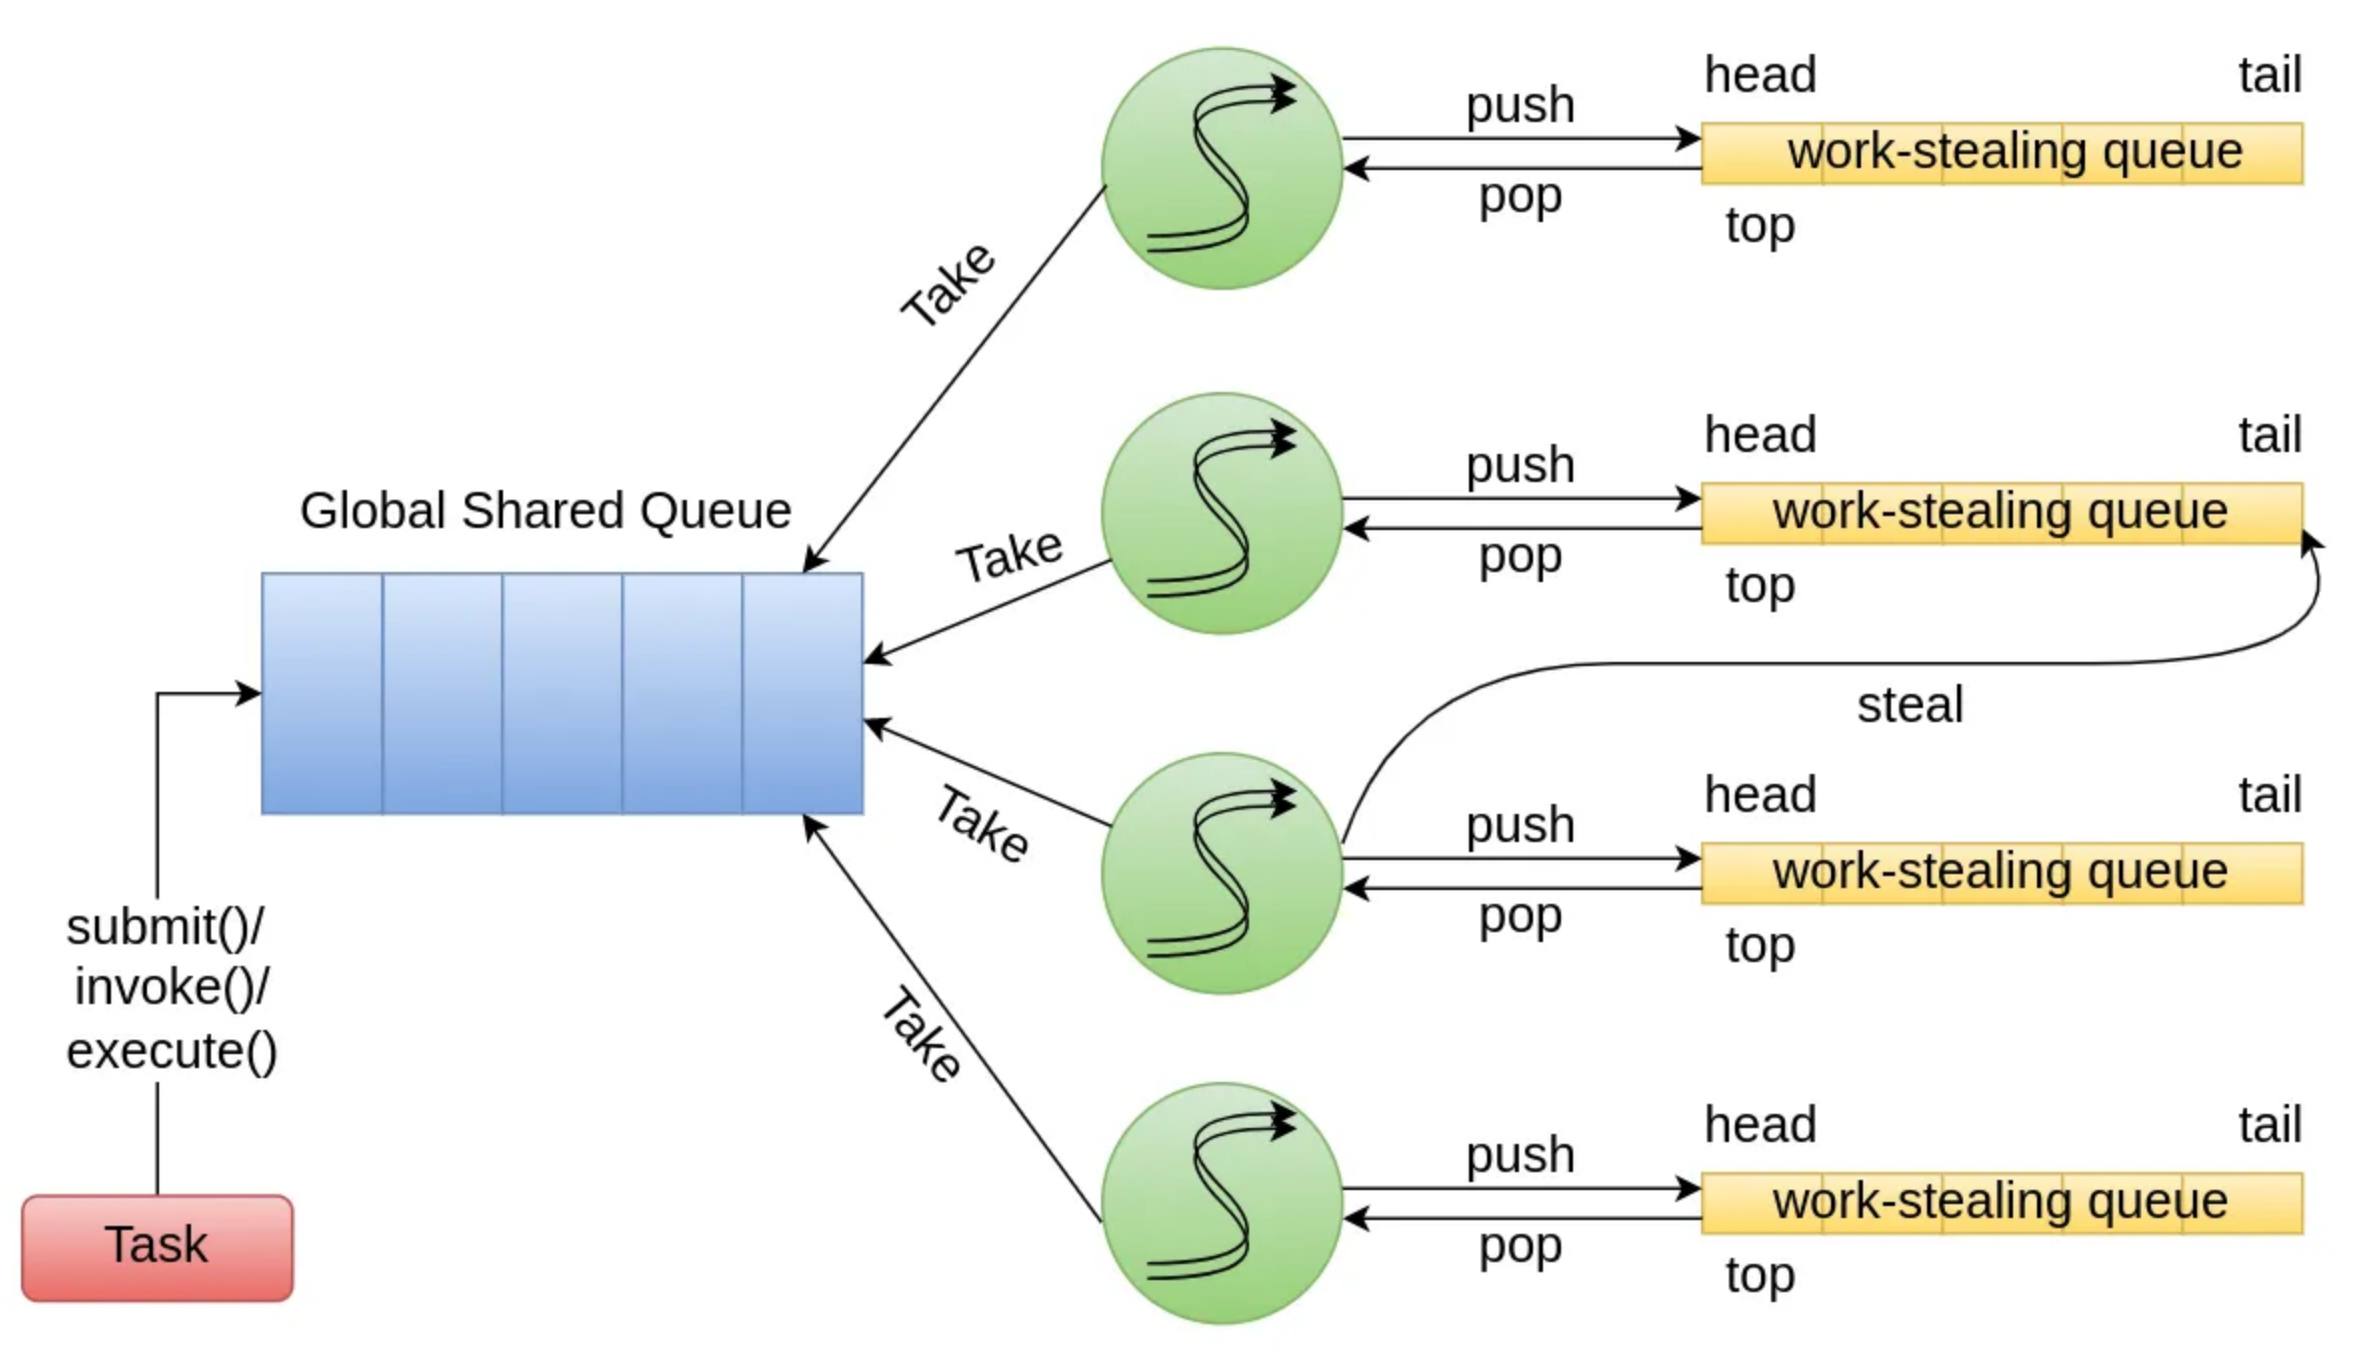
\includegraphics[scale=0.13]{ForkJoinQueues.png}
    \caption{Task distribution in a \texttt{ForkJoinPool} with four worker threads: https://krishnakishorev.medium.com/java-multithreading-concurrency-and-parallelism-part-22-3-9bc0429adc2b}
\end{figure}

\noindent Tasks submitted to the global queue can be taken by worker threads of the \texttt{ForkJoinPool}. Tasks that are \texttt{fork()}ed are directly pushed onto the executing thread's own queue (and not put into the global queue first). We can also see that threads steal tasks from the \textit{tail} of other queues, while they \textit{push} and \textit{pop} tasks to and from the \textit{head} of their own queue. This is an implementation detail to minimize collisions.

\subsubsection{Cilk}
Cilk is a programming language developed at MIT in the 1990s. Based on the C programming language, the idea behind Cilk was to extend C to better support multi-threaded programming. You might ask now why we even talk about Cilk in this course, as we already use Java. We are not concerned with actually learning the Cilk language or understanding its exact implementation details.\\
Cilk is relevant for us as it pioneered a specific programming style of spawning and joining tasks (i), using a work-stealing scheduler to map these tasks to available processors (ii), providing strong runtime guarantees based on this scheduling (iii) and introducing a multi-threaded computation model (iv). If you noticed that this sounds a lot like the Java fork/join framework, you are right. The fork/join framework in Java is based heavily on the Cilk language and thus we can learn a lot about it by studying the ideas behind Cilk.\\
The basis of Cilk-style programming is that the programmer expresses parallelism by spawning tasks and then joining them (waiting for results). A core of the project was to support fork/join parallelism by implementing a suitable task scheduler. The idea being that the programmer is concerned with the structure of the program (which tasks to spawn and join) and the scheduler is concerned with efficiently mapping these spawned tasks to available processors.


\subsubsubsection{The Cilk Model of Multi-Threaded Computation}
Closely tied to the Cilk programming style with spawning and joining tasks, Cilk also introduced a graph computation model that allows us to reason about runtime bounds. To introduce the model, we consider the following pseudo-code of the exponential Fibonacci algorithm:

\newpage

\begin{minted}[]{java}
public long fib(int n) {
    if (n < 2)
        return n;
    spawn task for fib(n-1);
    spawn task for fib(n-2);
    wait for tasks to complete
    return addition of results
}
\end{minted}

\noindent In the Java fork/join framework, the two spawns would correspond to \texttt{ForkJoinTask.fork()} operations and the wait to \texttt{ForkJoinTask.join()} operations.\\
We now consider the computation of \texttt{fib(4)}. We can model the program execution as a dag (directed acyclig graph) by:

\begin{itemize}
  \item Creating vertices for each \texttt{spawn} and \texttt{wait}.
  \item Grouping vertices within the same function call (for example within a call to \texttt{fib(3)}) into a \textbf{procedure} block.
  \item Creating a \textbf{spawn edge} for each spawn call, a \textbf{return edge} for each wait and a \textbf{continuation edge} for a step within the same function call (procedure).
\end{itemize}

\noindent We receive the following execution graph:

\begin{figure}[H]
    \centering
    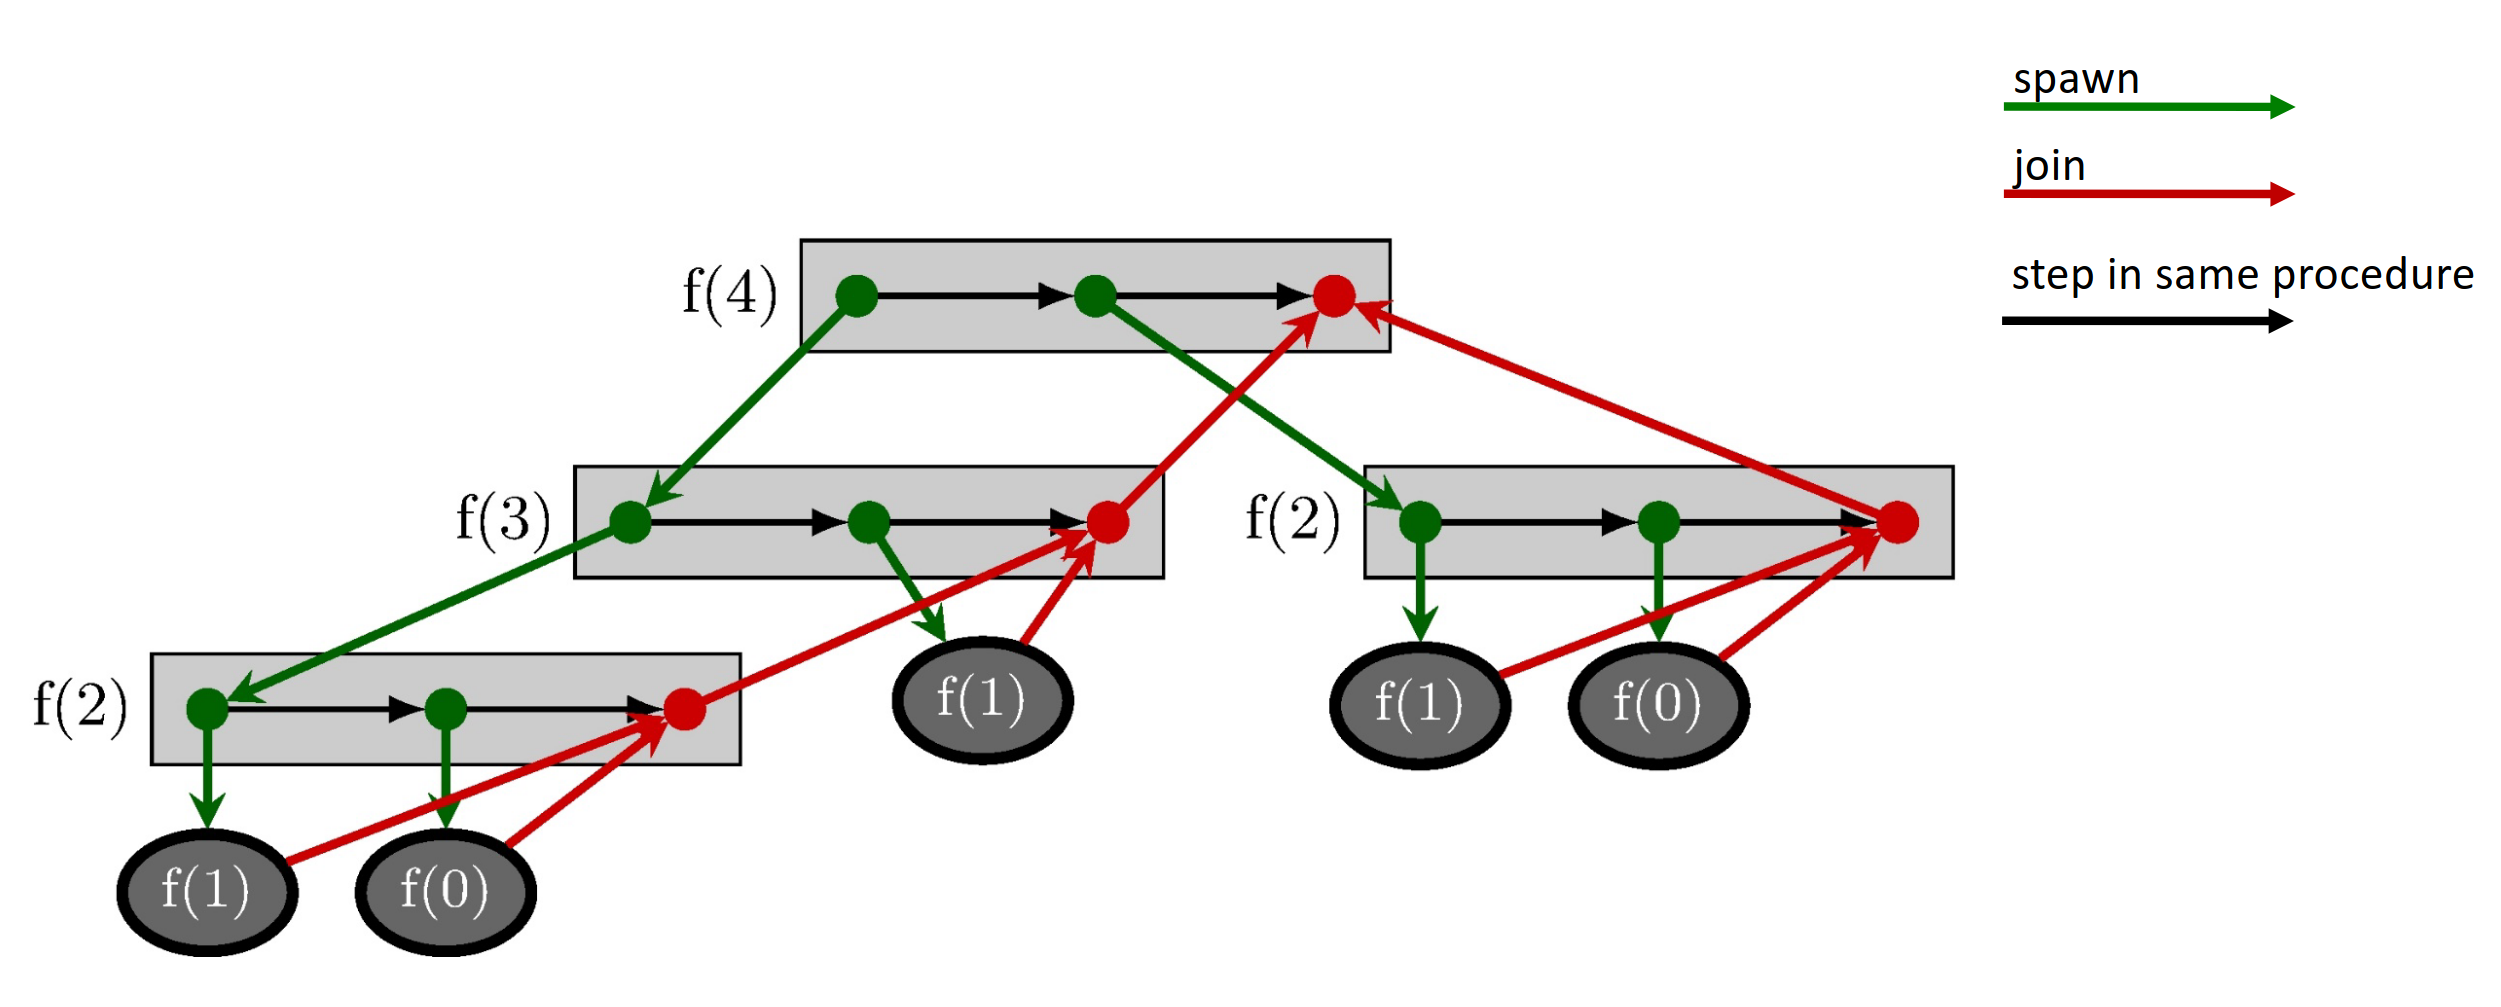
\includegraphics[scale=0.15]{FibTaskGraph.png}
    \caption{Cilk Graph of Fib(4) execution.}
\end{figure}

\noindent In each procedure (\texttt{Fib(n)} call), we have three vertices corresponding to two spawns and one wait. Exceptions are the leaves, which correspond to the base cases (\(n < 2\)) and thus immediately return without any vertices.

\subsubsubsection{Task Graphs}
The Cilk model of multi-threaded computation is an example of a task graph model. Such models help us visualize and understand dependencies in the code to see where we can exploit parallelism. We can simplify the Cilk model to model each procedure as a vertex and only model the spawn edges. The \texttt{Fib(4)} execution would then look like this:

\begin{figure}[H]
    \centering
    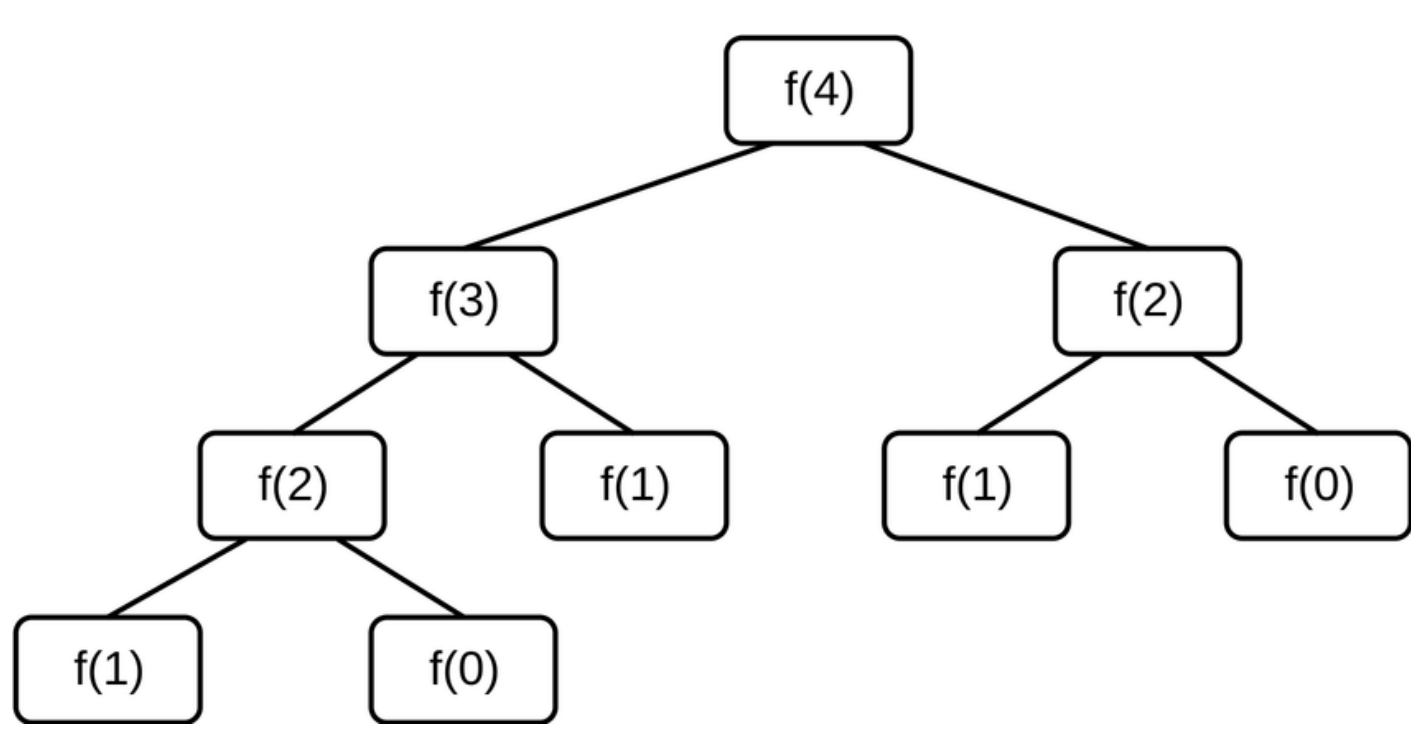
\includegraphics[scale=0.17]{FibSimpleTaskGraph.png}
    \caption{Simple Task Graph of Fib(4) execution.}
\end{figure}

\noindent With such a simple model, we sacrifice some precision in the dependencies, but we can reason about performance bounds in a more straight-forward manner.\\
Let us define that each vertex (task) takes one unit of time to execute. Then, \(T_{1} = n\), where n is the number of vertices in the task graph. This is because a single processor needs to sequentially execute one vertex after the other.\\
We can see that this kind of task graph is a dag. Branches of this dag have no dependencies between each other and could thus be executed in parallel. This also means that intuitively, the \textit{wider} the task graph, the more parallelism can be exploited.\\[3mm]
We notice that no matter how many processors we have, we are limited by the longest path in the graph. This is because each vertex in the path depends on its predecessor. Thus, each path (and in particular the longest path) has to be executed sequentially. Based on this observation, we can define the following:

\begin{definition}
  The \textbf{Critical Path} of a task graph is its longest path. The \textbf{Span} \(=T_{\infty}\) is the length of the critical path, that is, the time required to execute all vertices along the critical path.
\end{definition}

\noindent In our simple model where each vertex takes exactly one unit of time to execute, the span is thus simply the number of vertices lying on the longest path. In the case of our \texttt{Fib(4)} task graph, the span is four. With the span, we can define \textit{parallelism} within a task graph or program:

\begin{definition}
  \textbf{Parallelism} is the maximum possible speedup \(\frac{T_{1}}{T_{\infty}}\).
\end{definition}

\noindent This definition of parallelism formalizes our intuition that a wider task graph equates better parallelism, since a wider graph means more total vertices (i.e. \(T_{1}\) increases), but generally not more depth (i.e. \(T_{\infty}\) stays constant).\\[3mm]
With the definition of span we can also formulate the \textit{span law}:

\begin{theorem}
  \textbf{Span law}: \(T_{P}\geq T_{\infty}\)\\
  That is, any execution using P processors is lower bounded by the span of the task graph.
\end{theorem}

\noindent The law follows trivially from the fact that the span is equal to the execution time on an infinite number of processors \(T_{\infty}\) and thus any execution on any finite number of processors P cannot be faster than this.\\[3mm]
We can also formulate the \textit{work law}:

\begin{theorem}
  \textbf{Work law}: \(T_{P}\geq \frac{T_{1}}{P}\)\\
  That is, P processors require at least \(\frac{T_{1}}{P}\) time to execute all vertices in the task graph.
\end{theorem}

\noindent This is because in each unit of time, each processors can execute at most one vertex (due to dependencies, it might be less than one per processors).\\
We can only give bounds on \(T_{p}\) because it depends on how we schedule the vertices (tasks) on the available number of processors. Let us illustrate this on the following task graph:

\begin{figure}[H]
    \centering
    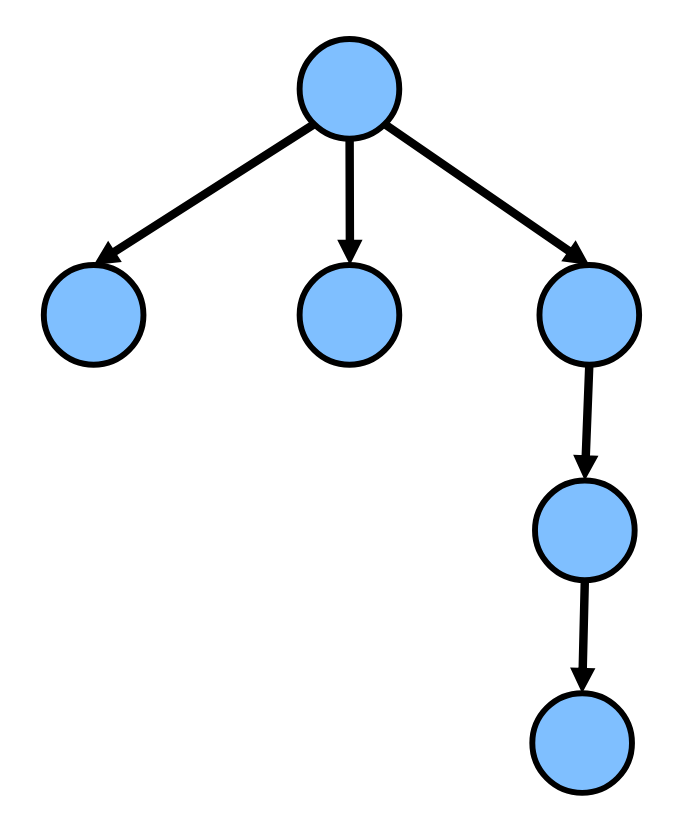
\includegraphics[scale=0.17]{ScheduleTaskGraph.png}
\end{figure}

\noindent What is \(T_{2}\) here? Using our previously deduced bounds, the \textit{work law} tells us that \(T_{2}\geq \frac{6}{2}=3\) since \(T_{1}=6\) and the \textit{span law} tells us that \(T_{2}\geq 4\), since the critical path has length four. However, the exact value of \(T_{2}\) depends on the scheduling we choose. Consider the following two possible schedulings:

\begin{figure}[H]
    \begin{subfigure}[t]{.5\textwidth}
        \centering
        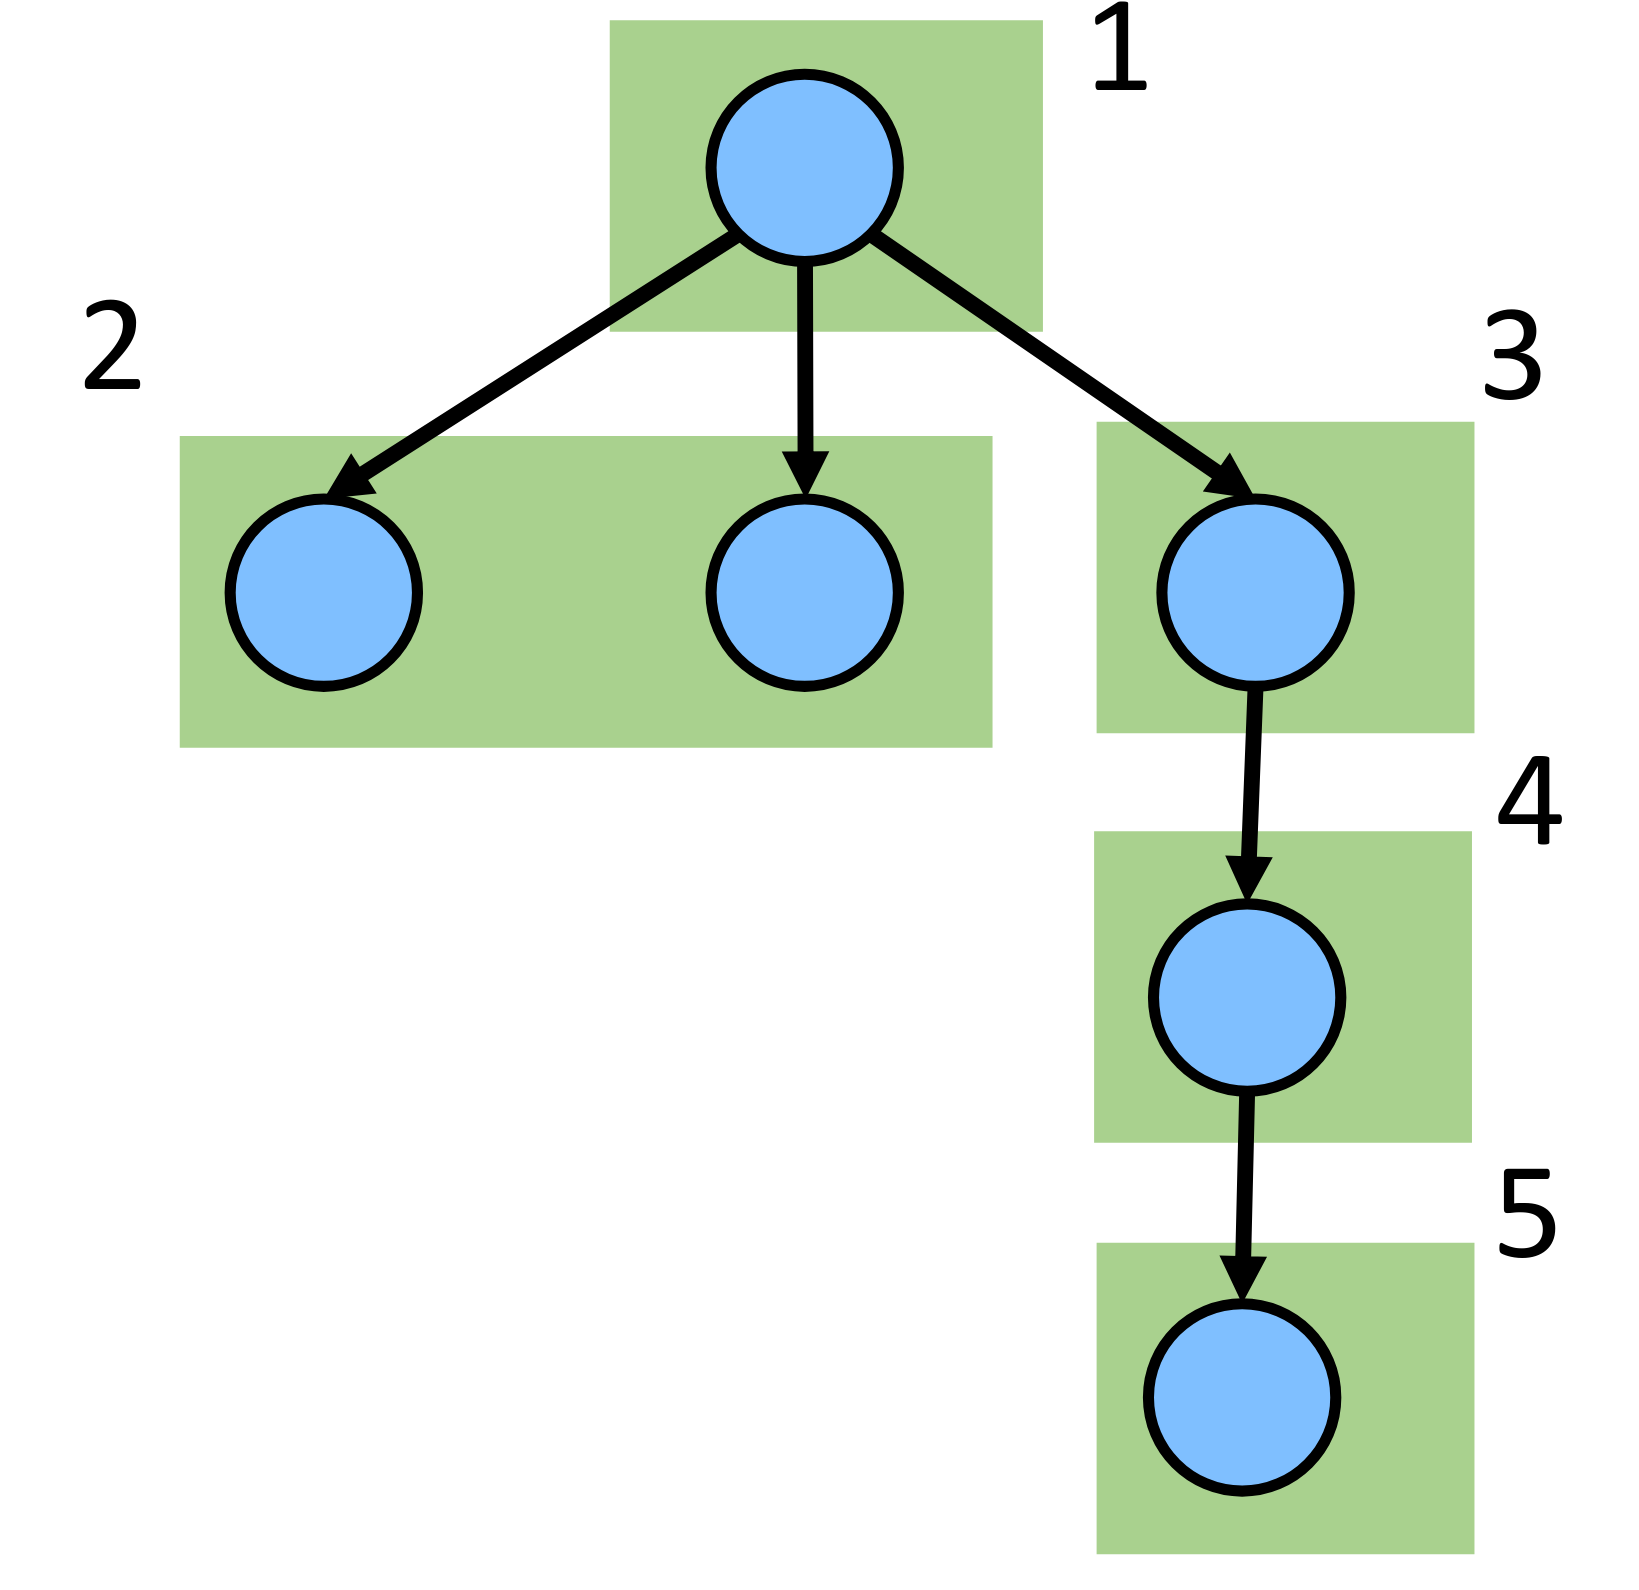
\includegraphics[scale=0.1]{Schedule1.png}
    \end{subfigure}
    \begin{subfigure}[t]{.5\textwidth}
        \centering
        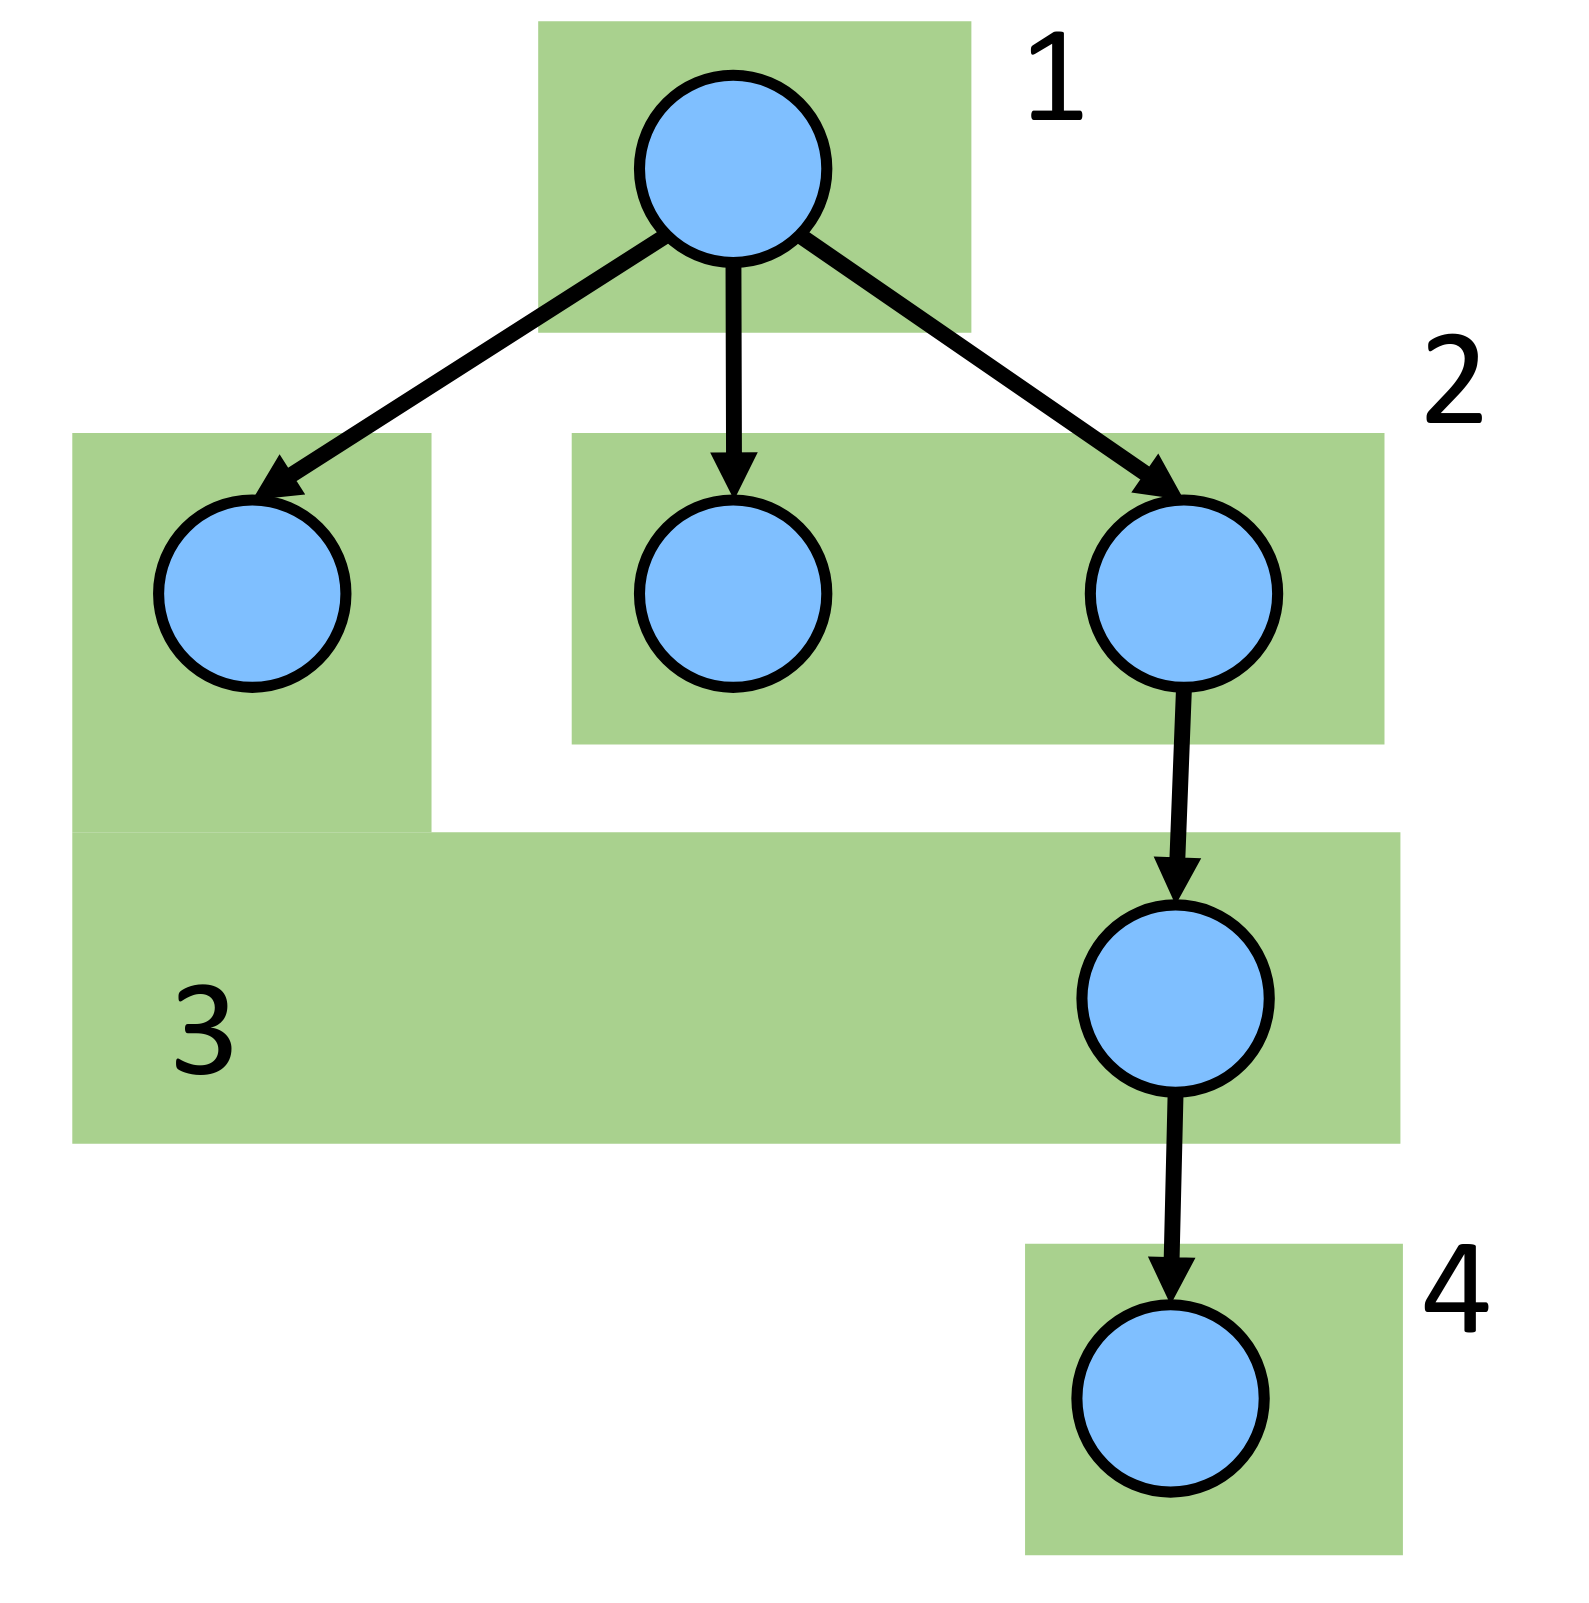
\includegraphics[scale=0.1]{Schedule2.png}
    \end{subfigure}
\end{figure}

\noindent In the first case, we can only exploit the second processor in the second time step. With this scheduling, \(T_{2}=5\). However, with the second scheduling, \(T_{2}=4\), which is optimal according to the span law.

\subsubsubsection{Runtime Guarantees of Cilk}
To get back to the subject matter, why did we introduce task graphs in this part of the course? Cilk introduced its task graph model in order to be able to prove theorems and thus provide guarantees about the execution of its programs.\\
In the previous section, we learned that \(T_{P}\) depends on the scheduling. A core of the Cilk language is its work-stealing scheduler that can provide strong runtime guarantees that are provable within this task graph model. In particular, Cilk gives us the following guarantee about the execution time on P processors:
$$\mathbb{E}(T_{P})=\mathcal{O}\left(\frac{T_{1}}{P} + T_{\infty}\right)$$
\noindent That is, the expected time required to execute a Cilk program on P processors is equal to the critical path length \(T_{\infty}\) plus the sequential time \(T_{1}\) divided by the number of processors P. This is a strong guarantee, as both \(T_{\infty}\) and \(\frac{T_{1}}{P}\) are lower bounds on any parallel execution (span law and work law).\\
This means that a Cilk program has an expected runtime that is within a constant factor of optimal. The guarantee can only be given with regards to the expected value (and not about worst-case), because the work-stealing algorithm employs some randomization (for example randomizing which thread to steal work from). Of course we know that the O-notation can hide enormous constants. However, empirical testing showed that the runtime of Cilk programs is very close to optimal with small constants, that is, \(T_{p}\approx \frac{T_{1}}{P}+T_{\infty}\).\\
The important part for us in this course is that the Java fork/join framework is based on Cilk, adopting both its spawning/joining programming style and its work-stealing scheduler, thus also inheriting this strong runtime guarantee.

\subsubsection{Summary: Fork/Join Programming in Java}
After an odyssey where we...
\begin{enumerate}
  \item Recognized the \textbf{value of parallel divide-and-conquer} due to the simple program structure, ability to easily implement effective load balancing and ability to parallelize even the result combination.
  \item Recognized that using \textbf{Java threads for fork/join is not optimal}, since they block resources (memory, OS threads) and bring a lot of overhead (bookkeeping, context switching). To solve all these problems, we stumbled upon the \texttt{ExecutorService} framework, that offers light-weight tasks instead of heavy-weight threads. We had to notice that the fixed thread pool of the \texttt{ExecutorService} is not designed for recursion.
  \item Found that the \textbf{Java fork/join framework} is exactly what we were looking for and enables us to reap all the benefits we originally hoped for from implementing parallel divide-and-conquer.
  \item Learned how the \textbf{Cilk programming language} pioneered multi-threading in programming languages and contributed a work-stealing scheduler enabling efficient fork/join parallelism that inspired Java to adopt most of its features within the fork/join framework. We learned that by modelling programs with task graphs, Cilk manages to prove asymptotic lower bounds on execution time that thus also apply to the Java fork/join framework.
\end{enumerate}
... we might feel a bit lost about where we end up now. We have not yet actually learned how to systematically parallelize algorithms, but we have acquired a critical tool towards implementing them efficiently in general (with the programming style of forking and joining tasks) and in particular using the fork/join framework in Java. In the case of the fork/join framework, we even have the guarantee that our programs will run in asymptotically optimal expected time (in the number of processors P) \(\mathbb{E}(T_{P})=\mathcal{O}\left(\frac{T_{1}}{P} + T_{\infty}\right)\) which gives us a solid foundation to write parallel algorithms on.\\
We also learned how to model parallel programs using task graphs. This helps us think about the parallelism of programs more easily and enables the distinction between work (\(T_{1}\)) and span (\(T_{\infty}\)). Our goal for parallel algorithms in terms of performance is thus to reduce span in particular.

\subsection{Parallel Patterns}
Now we can finally talk about parallelizing algorithms. To be able to do so systematically, we need to look out for patterns in our code. Some important patterns are introduced in this section.

\subsubsection{Maps and Reductions}
We start with the two most straightforward and also most common patterns and add complexity later.

\subsubsubsection{Reductions}
Remember all the work we had to do in order to parallelize array summation using the fork/join framework in Java? The good news is that many problems can be effectively parallelized almost exactly like our array summation. Here are a few problems that can be efficiently parallelized using an approach almost exactly to our divide-and-conquer array summation:

\begin{itemize}
  \item Return the maximum or minimum element of an array.
  \item Return the number of elements in an array that fulfill some property.
  \item Return the leftmost element of an array fulfilling some property.
\end{itemize}

\noindent The only parts about the fork/join algorithm that are subject to change are the base case and the combination of results. So, say we want to return the number of elements fulfilling some property:

\begin{itemize}
  \item For the base case, return 1 if array[startIdx] fulfills the property and 0 otherwise. If we implement a cutoff, which is more efficient, simply loop over the assigned chunk (of about 1000 elements) and count how many elements fulfill the property.
  \item To combine the two joined subtasks, simply add the results.
\end{itemize}

\noindent Problems of this form are called \textbf{reductions}. A reduction is an operation that produces a \textit{single} answer from a collection (for example an array or linked list) via an \textit{associative} operator. This single answer can for example be a count, an element of the collection itself, a boolean value or even something like a histogram. The associativity of the operation is important such that even when dividing and recombining partial results, the end result does not change. If the operation was not associative, we could not use a divide-and-conquer strategy.

\subsubsubsection{Maps}
A \textbf{map} is an operation characterized by two properties:

\begin{enumerate}
  \item A map operates on each element of a collection (for example an array or a linked list) independently.
  \item A map outputs a new collection of the same size.
\end{enumerate}

\noindent An operation that fulfills this is for instance vector addition. We start with a vector X and add a vector Y (of the same size) to it. This operates on each element of X independently and results in a new vector Z of the same size as X. Note that we do not perform the \textit{same} operation on each element of X (to each X[i], we add Y[i], which is presumably different for each i), but this is not a requirement of a map operation.\\
Maps are often called \textit{embarrasingly parallel}, since each element can be processed independently by definition and thus parallelizing a map is trivial.\\
We can implement maps using the fork/join framework as well. Consider again vector addition. To plan out how we use the fork/join framework to parallelize this, we consider the following:

\begin{enumerate}
  \item For the \texttt{ForkJoinTask} class, we choose to subclass \texttt{RecursiveAction} (instead of \texttt{RecursiveTask<T>}) since working with an array reference is more efficient than actually returning an array copy. So, we do not need a return value.
  \item For the \texttt{RecursiveAction} class, we need to store the two input arrays, a result array, a start index and an end index.
  \item The base case is simply a for loop to sequentially sum the assigned array chunk (defined by start index and end index).
  \item For the recursion, we simply need to fork two tasks to sum each half of the assigned chunk. We do not need to combine these result in any way.
\end{enumerate}

\noindent Based on this, we write the following \texttt{RecursiveAction} subclass:

\begin{minted}[]{java}
class VecAdd extends RecursiveAction {
    private final int SEQUENTIAL_CUTOFF = 1000;
    private int startIdx, endIdx;
    private double[] res, arr1, arr2;

    // constructor
    VecAdd(int startIdx, int endIdx, double[] res, double[] arr1, double[] arr2) {
        this.startIdx = startIdx;
        this.endIdx = endIdx;
        this.res = res;
        this.arr1 = arr1;
        this.arr2 = arr2;
    }

    protected void compute() {
        if (endIdx - startIdx <= SEQUENTIAL_CUTOFF) {
            for (int i = startIdx; i < endIdx; i++)
                res[i] = arr1[i] + arr2[i];
        } else {
            int mid = (endIdx + startIdx) / 2;
            VecAdd left = new VecAdd(startIdx, mid, res, arr1, arr2);
            VecAdd right = new VecAdd(mid, endIdx, res, arr1, arr2);
            left.fork();
            right.fork();
            left.join();
            right.join();
        }
    }
}
\end{minted}

\noindent To perform vector additions now, we can write the following method where we initialize a \texttt{ForkJoinPool} and start the initial task:

\begin{minted}[]{java}
public double[] vectorAdd(double[] arr1, double[] arr2) {
    double[] res = new double[arr1.length]; // initialize empty result array
    ForkJoinPool fj = new ForkJoinPool();
    RecursiveAction vec = new VecAdd(0, arr1.length, res, arr1, arr2);
    fj.invoke(vec);
    fj.shutdown();
    return res;
}
\end{minted}

\noindent This is just a reminder on how to use the fork/join framework. We see that implementing maps is very straightforward and even simpler than implementing reductions, because we do not need to combine the partial results of the subtasks.

\subsubsubsection{Digression: Map/Reduce vs Fork/Join in Distributed Systems}
We may now think that we have a clear hierarchy, where maps and reductions are high-level patterns that can be exploited by means of fork/join-style programming. However, there is a paradigm called map/reduce that is based on maps and reductions, although it views maps and reductions a bit differently. Map/reduce is the basis of computing in distributed systems, while fork/join is utilized mostly on shared memory systems. Let us elaborate on the difference between these two terms:

In this course, we focus almost solely on parallel programming within a single computer in a shared memory environment. This means that the different entities partaking in the parallel computing (the processors/cores) share memory and can thus efficiently communicate with each other. There is also \textit{distributed computing} operating on a larger scale with massive datasets, where the entities are called nodes and are usually whole computers. There is no shared memory between the nodes (communication happens by sending messages and is expensive) and data is distributed as well (each node has some part of the data while in shared memory computing, all processors can access the entire data). Hence the paradigms used to parallelize computations are different. While in shared memory computing, fork/join parallelism is popular, map/reduce is the workhorse of distributed computing.

To understand why fork/join does not make so much sense in distributed computing, let us introduce an analogy. We can think of the distributed computing environment as the Holy Roman Empire, where we want to conduct a concensus. The data we operate on are the citizens and each city can be considered a node. The data is not shared, as each city can only count its own inhabitants. So, we would let each city locally count its inhabitants (all cities in parallel) and then let them send their results back to the capital, where the partial results are summed (or \textit{reduced}) to the final answer. Generally, everything that can be computed per node is considered a map in distributed map/reduce (even though not strictly a map according to our definition) and only when we have to combine the partial results of each node we call it a reduction.

A divide-and-conquer approach would not make much sense here. Cities would have to exchange their results with each other and sum them, but considerable distances would have to be covered to communicate these results between cities. It requires much less communication and is more efficient to just let each city send a representative to the capital once. Note however that each city can be considered a shared memory environment itself and can parallelize its local counting (where communication is cheaper) using a divide-and-conquer approach.

This example is not a perfect analogy, but it gives us sufficient intuition on why fork/join and map/reduce coexist as paradigms - they are designed to exploit parallelism in different environments and on a different scale.\\[3mm]
To conclude, map/reduce makes sense as a paradigm in distributed systems since communication between nodes is expensive and should be minimized. Hence, divide-and-conquer is usually not efficient. Instead, a more course-grained approach towards parallelism is taken by dividing large datasets on different computers (or nodes), letting each operate on its own chunk of data (to perform maps and generate partial results) and when its necessary reduce these partial results to a single node again.

\subsubsubsection{Stencil}
A stencil is a generalization of a map. Remember that we had two criteria for a map; it needs to be applied to each element of a collection independently and it needs to result in a collection of the same size. A stencil relaxes the first condition and allows the function to take more than one element of the collection as an input.

Stencils are often used in image processing in the form of filters. The canonical example is a median filter over an image, where the input and output is a two-dimensional array. The (i,j)'th entry of the output is the median value of the (i,j)'th entry and its surrounding values in the input matrix.

\begin{figure}[H]
    \centering
    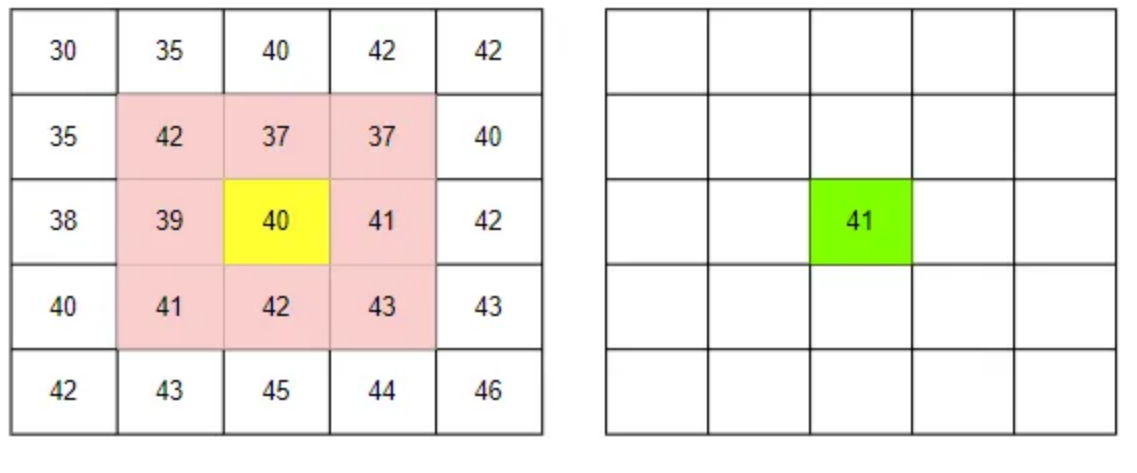
\includegraphics[scale=0.2]{AverageFilter.png}
    \caption{In Green is the Output Value corresponding to the Yellow Input Value and its Surrounding: https://miro.medium.com/v2/resize:fit:1148/format:webp/1*-NVjiEYLFVOdRbxkihA8Qg.png}
\end{figure}

Stencils can be parallelized just as maps, since each output element can be computed independently. We need to make sure to not perform the computation in-place, else we might read elements as input that are actually already computed output. So, usually, the result needs to be a new collection.

\subsubsection{Scan}
A scan is a pattern, where:

\begin{itemize}
  \item We are given a collection A and need to return a collection B.
  \item We are given a function f and the output B is computed according to the rule \(B[i] = f(B[i-1], A[i])\).
        \item This rule is equivalent to the following: \(B[i] = f(A[i], f(A[i-1], ... , f(A[0], b_{0})))\). \(b_{0}\) is some initial given value.
\end{itemize}

\noindent We can visualize this in the following way:

\begin{figure}[H]
    \centering
    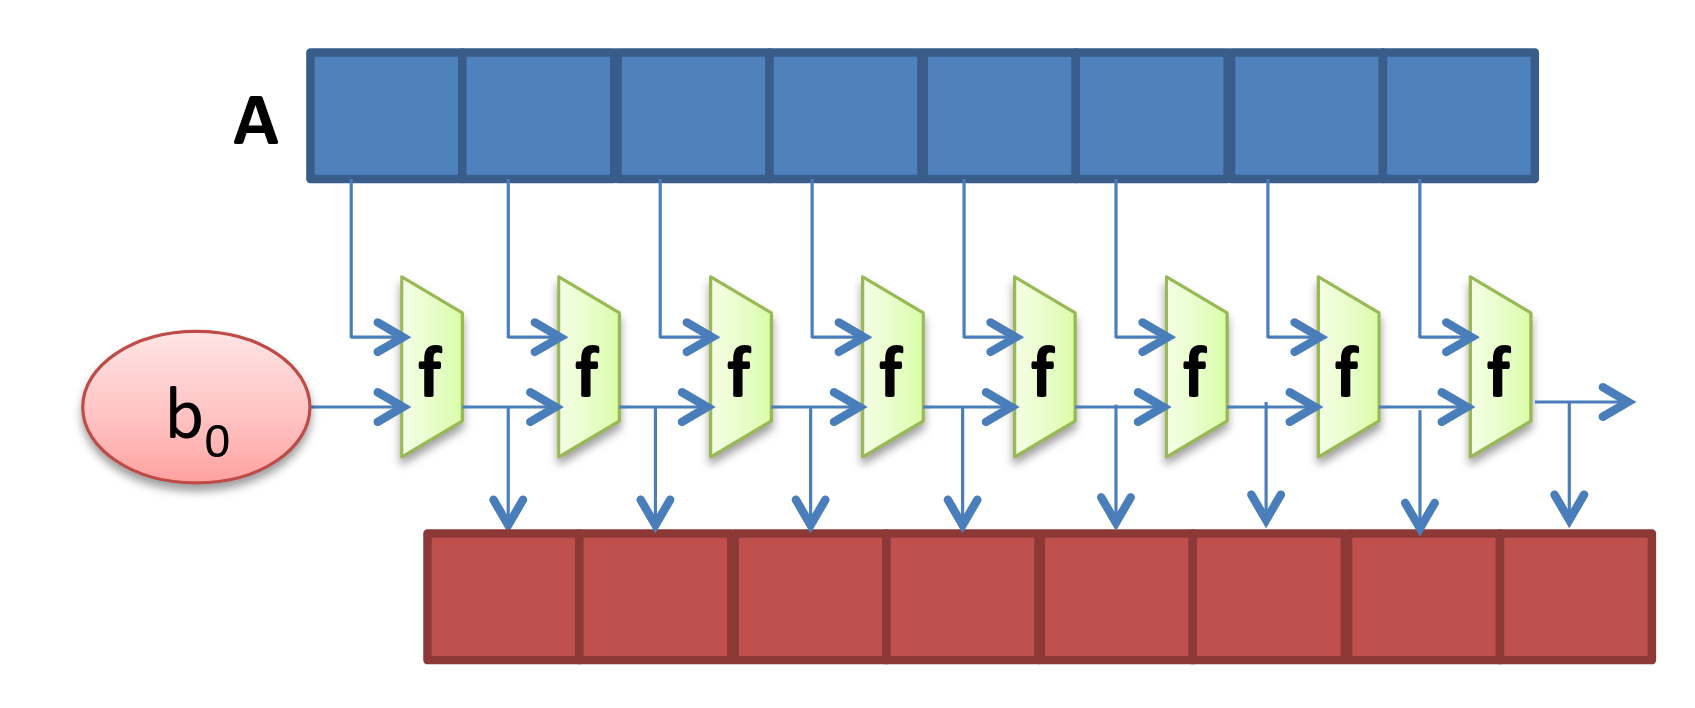
\includegraphics[scale=0.15]{Scan.png}
\end{figure}

\noindent While the pattern is similar to a reduction, it seems inherently sequential. However, we will see that we can efficiently parallelize scan patterns where f is associative (because then we can implement a divide-and-conquer version) to get a \(\mathcal{O}(log(n))\) span.

\subsubsubsection{Scan Example: Parallel Prefix Sum}
To get a better feeling for the pattern, we proceed with an example. Consider the prefix-sum problem, where we are given an input array and need to return an output array defined as:
$$output[i]\ =\ \sum_{k=0}^{i}input[k]$$
Here, we have \(f(x,y)=x+y\) and \(b_{0}= 0\). A sequential Java implementation of the prefix-sum problem looks like this:

\begin{minted}[]{java}
public int[] prefix_sum(int[] input){
    int[] output = new int[input.length];
    output[0] = input[0];
    for(int i=1; i < input.length; i++)
        output[i] = output[i-1] + input[i];
    return output;
}
\end{minted}

\subsubsubsection{Parallelizing the Prefix Sum Algorithm}
\noindent The span of this implementation is \(\mathcal{O}(n)\), which allows for no parallelism. Let us try to improve upon it by using a divide-and-conquer approach. Assume we have an array of eight elements. Sequential prefix sum has a critical path containing seven additions. Imagine now we divide this array in two halves for which we compute their prefix-sum in parallel:

\begin{figure}[H]
    \centering
    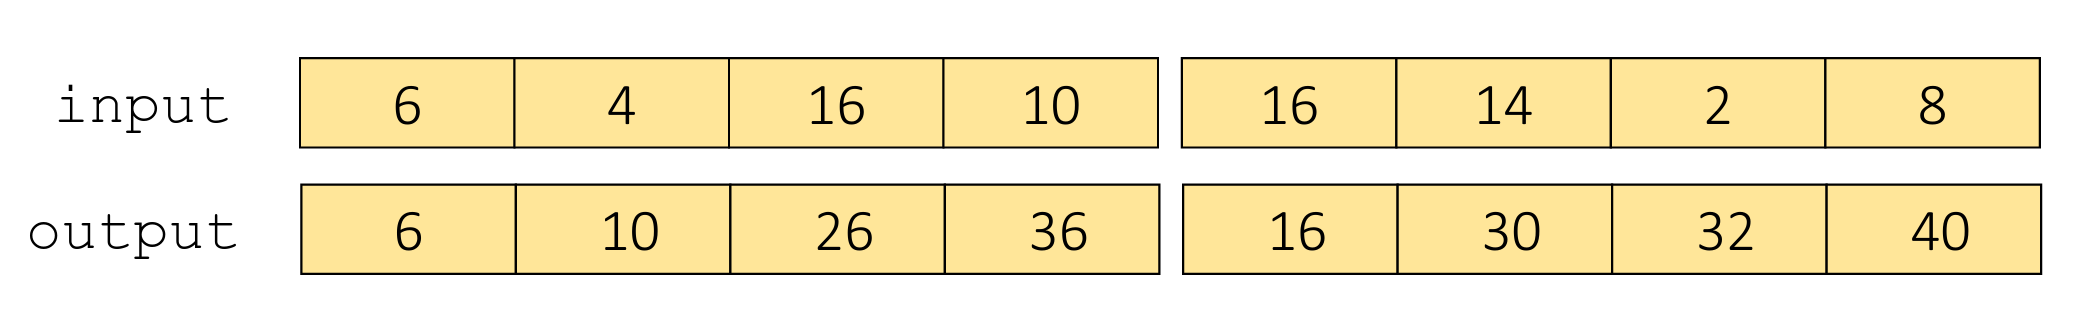
\includegraphics[scale=0.15]{PrefixSum1.png}
    % \caption{Prefix Sum with Halving Once.}
\end{figure}

\noindent Both halves require three additions, which we can perform in parallel. In order to fix the result of the right half, we need to add 36 to each element. These four additions are independent though and can be performed in parallel. Hence, the critical path contains only four additions. With this fix, we receive the correct result:

\begin{figure}[H]
    \centering
    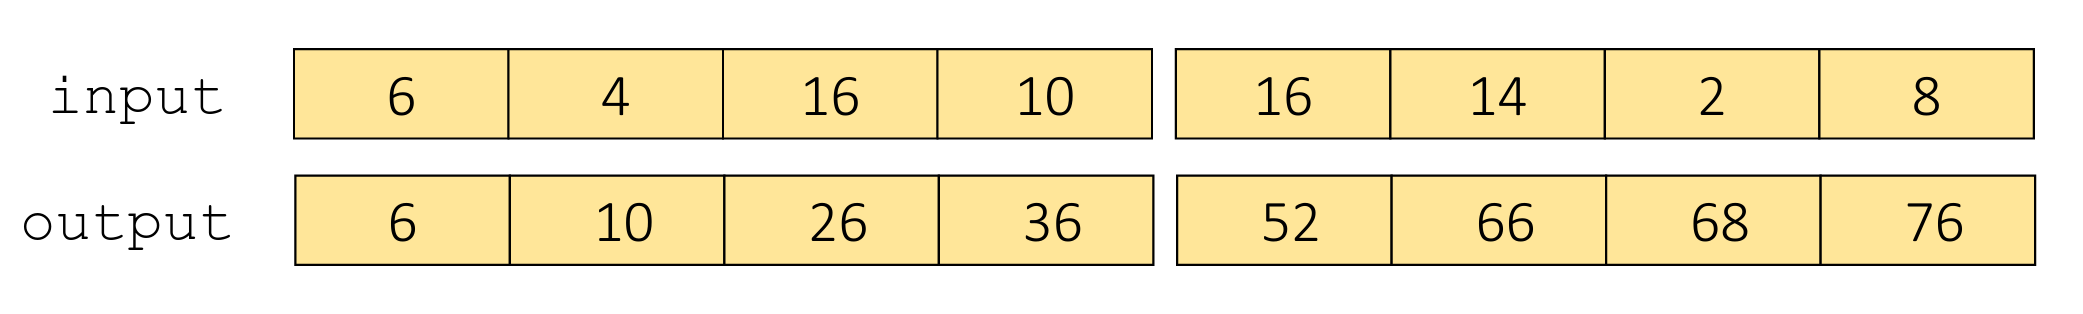
\includegraphics[scale=0.15]{PrefixSum2.png}
    % \caption{Prefix Sum with Halving Once.}
\end{figure}

\noindent Continuing the algorithm, let us try to write this as a classical divide-and-conquer algorithm, i.e. think about what the base case is and how to combine the partial results:

\begin{itemize}
  \item The base case is the usual; a for loop sequentially computing the prefix sum for the assigned chunk. We already wrote the code for this above. This will compute the \textit{local} prefix sum, in the sense that this will need to be corrected by adding the sum of all elements left of the assigned chunk. We need to think about this correction in the recursion.
  \item For the recursion, we need to fork and join a task for each half of the assigned chunk to compute the (local) prefix sum. But what do we need to do to combine the two results? We need to correct the right half somehow. The left half is okay, but to each element in the right half, we need to add the sum of all elements in the left half. Doing this sequentially means \(\mathcal{O}(n)\) to combine results unfortunately, leading to an overall \(\mathcal{O}(n)\) span. However, we want \(\mathcal{O}(log(n))\). We cannot do this in a single pass.
\end{itemize}

\noindent We conclude that we have to do the computation in two passes. The plan is that the first pass computes the local prefix sums and the second pass adds the corrections. Two passes in both \(\mathcal{O}(log(n))\) span means the overall span will still be in \(\mathcal{O}(log(n))\). But now, how do we execute the second pass to correct the results? Let us think about \textit{when} we need to add a correction:

When we initially split the array into two, we do not need to add a correction to the left chunk, since no array elements are to the left of it. But, to the elements of the right chunk, we will need to add the sum of all the elements of the left chunk. The beauty of recursion is that this happens again every time we further split the array. We always need to add the previous correction plus the sum of the elements of the chunk assigned to the left subtask. Let us draw the resulting computation tree on our previous example to understand what is going on:

\begin{figure}[H]
    \centering
    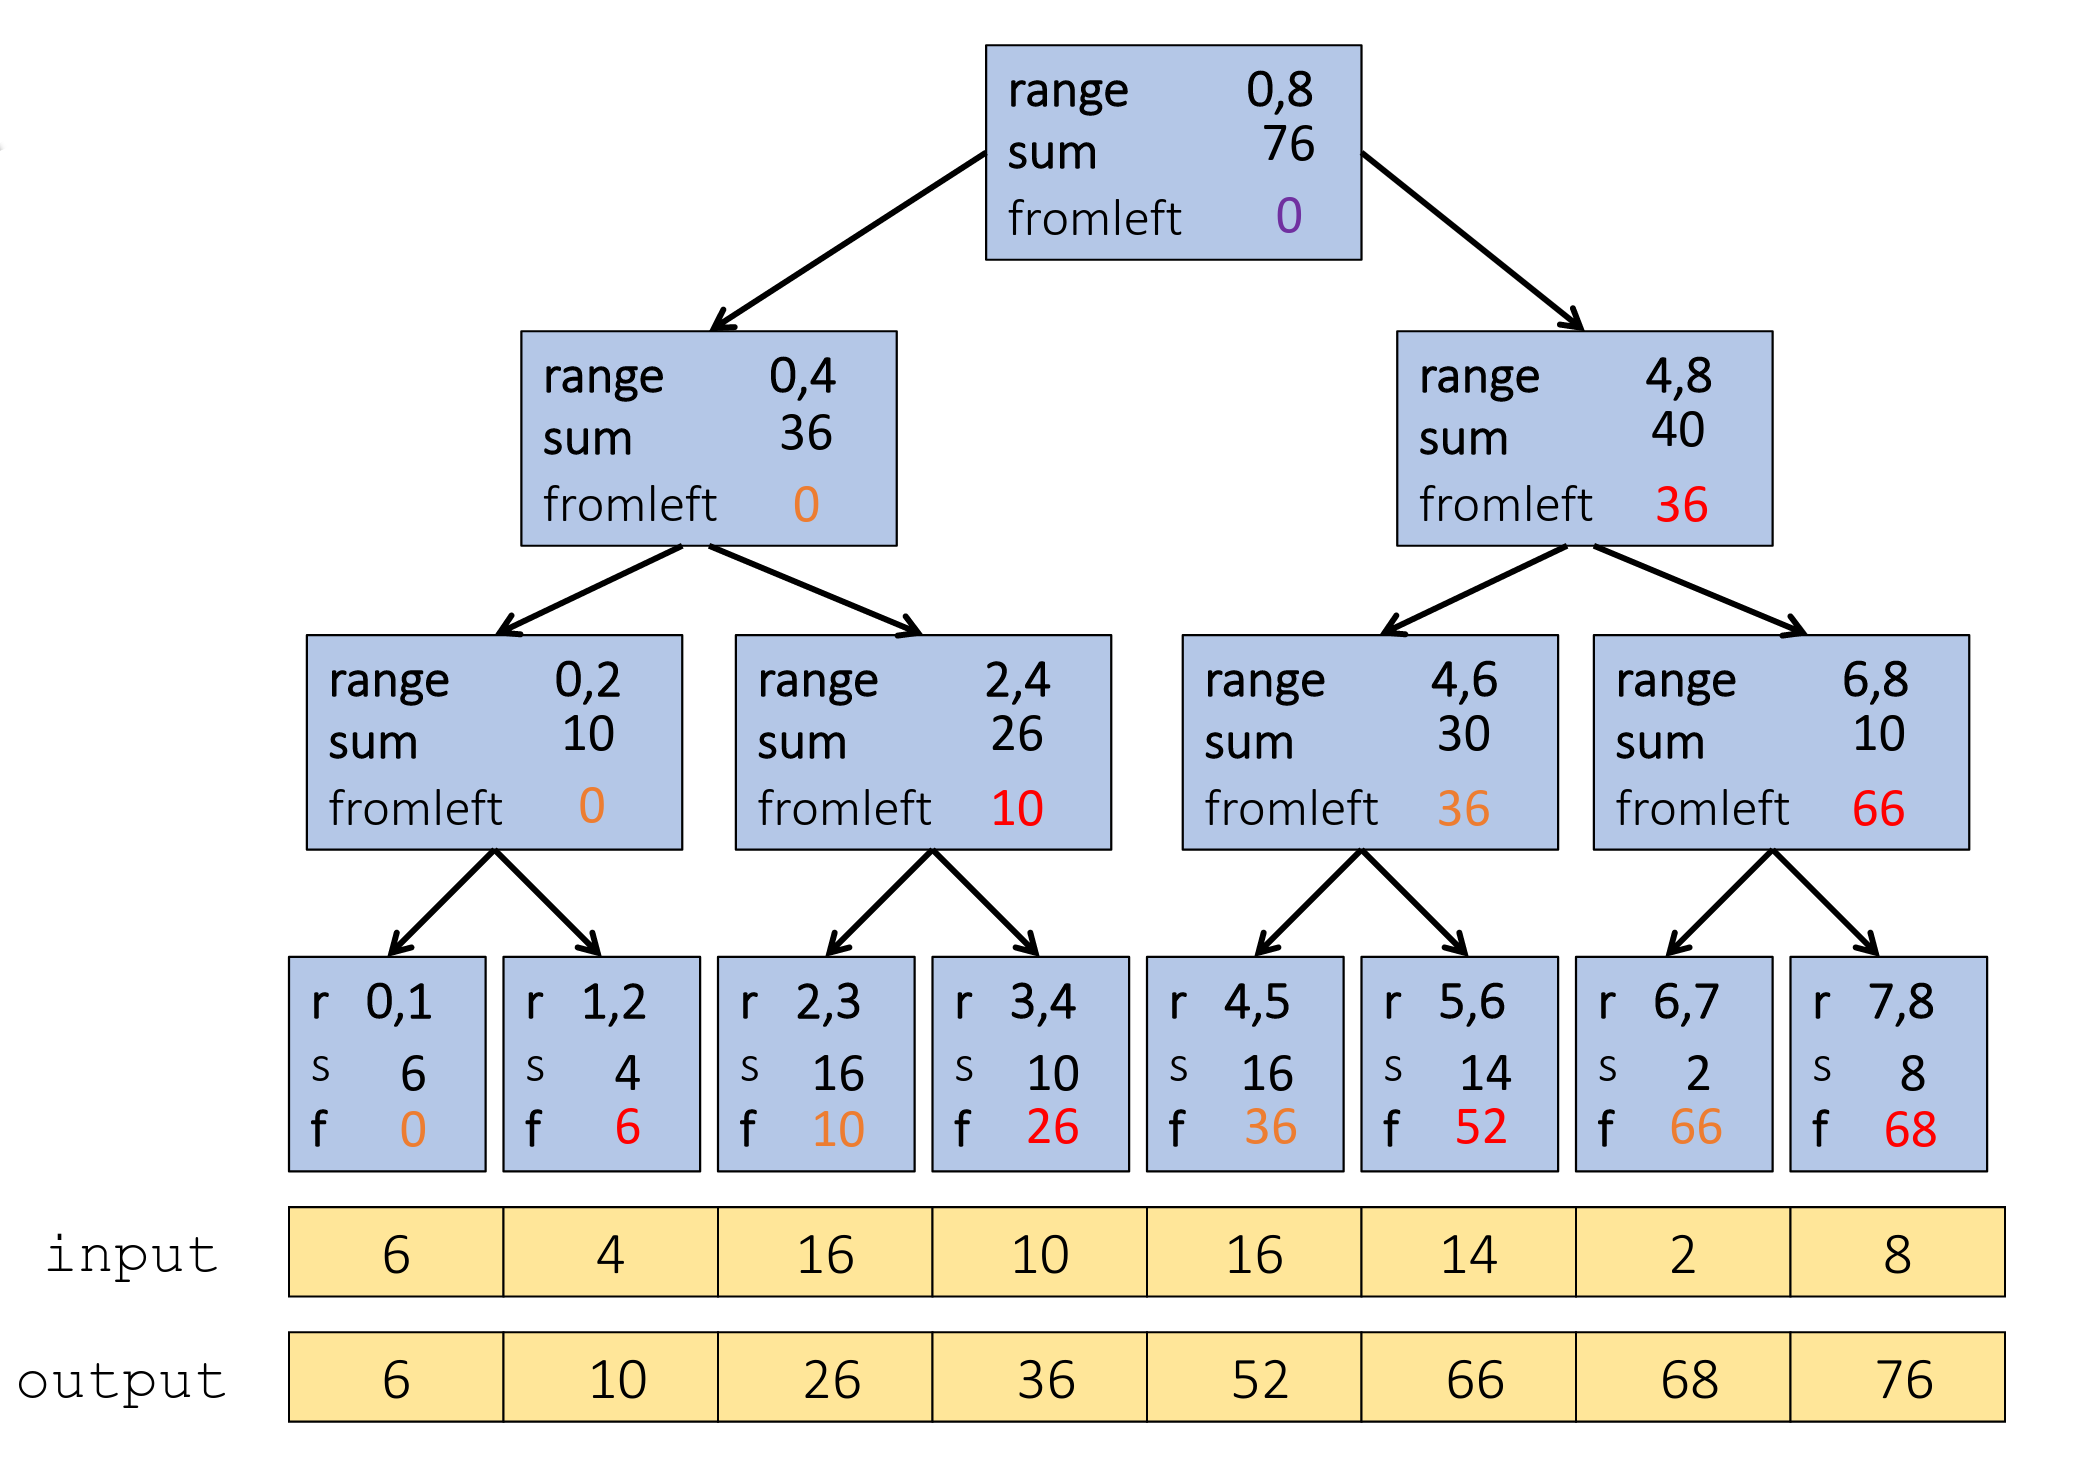
\includegraphics[scale=0.16]{PrefixSumTree.png}
    % \caption{Structure of a Divide-and-Conquer Program.}
\end{figure}

\noindent The nodes of our computation tree are the tasks created. The \texttt{fromleft} field is the correction we need to apply. Remember that we said that the left subtask will not need to do additional correction, so a task can pass on its correction to the left subtask. To the right subtask however, it will need to add the sum of all elements in the range of the left subtask. When each node (or task) stores the sum of all the elements in its range, the correction can be done in the second pass using the following divide-and-conquer pattern:

\newpage

\begin{minted}[]{java}
if (end - start <= CUTOFF) {
    for (int i = start; i < end; i++) {
        resultArray[i] += correction;
    }
} else {
    int mid = (start + end) / 2;

    SecondPass left = new SecondPass(resultArray, correction, start, mid);
    SecondPass right = new SecondPass(resultArray, correction + sumOfLeftSubtask, mid, end);
    left.fork();
    right.fork();
    left.join();
    right.join();
}
\end{minted}

\noindent The important things here are that we pass on the same correction to the left subtask and the correction plus \texttt{sumOfLeftSubtask} to the right subtask. This is more or less the final code for the second pass. However, in order to get \texttt{sumOfLeftSubtask}, we need to compute it in the first pass and store it somewhere for the second pass to find it.

So, let us now think about the first pass. We need to compute the local prefix sums, which we can simply do in the base case, nothing to do in the recursion. But we now also want to compute the sum of all elements in the range. This is the exact fork/join algorithm of summing up an array we previously implemented. Now we need to store this sum somewhere for each node in the computation tree. We can simply do this by \textit{flattening} the tree into an array, just like with a heap. That is, we store the result of the first task (the root of the tree) at index 0. When a task stores its result at index i, its children will store it at indices \((2*i)+1\) and \((2*i)+2\) respectively. In the second pass, we can simply access these same indices again to retrieve the sums. Let us write the compute method of the first pass task:

\begin{minted}[]{java}
class FirstPass extends RecursiveTask<Integer> {
    private final int CUTOFF = 1000;
    private int[] arr, res;
    private int start, end, id;

    FirstPass(int[] arr, int[] res, int start, int end, int id) {
        this.arr = arr;
        this.res = res;
        this.start = start;
        this.end = end;
        this.id = id;
    }

    protected Integer compute() {
        if (end - start <= CUTOFF) {
            int sum = arr[start];
            res[start] = arr[start];
            for (int i = start + 1; i < end; i++) {
                res[i] = res[i - 1] + arr[i]; // compute the (local) prefix sum
                sum += arr[i]; // compute the sum of the assigned elements
            }

            sums[id] = sum;
            return sum;
        } else {
            int mid = (start + end) / 2;

            FirstPass left = new FirstPass(arr, res, start, mid, 2 * id + 1);
            FirstPass right = new FirstPass(arr, res, mid, end, 2 * id + 2);
            left.fork();
            right.fork();
            int leftSum = left.join();
            int rightSum = right.join();

            sums[id] = leftSum + rightSum; // write the sum into an array
            return leftSum + rightSum;
        }
    }
}
\end{minted}

\noindent The code is almost the same as the recursive array sum algorithm. The difference being that in the base case, we also compute the local prefix sum, we write the sum into a \texttt{sums} array and we also give the tasks an \texttt{id}. This is the final version of the first pass and we can now finally write the final version of the second pass:

\begin{minted}[]{java}
class SecondPass extends RecursiveAction {
    private final int CUTOFF = 1000;
    private int[] res;
    private int start, end, correction, id;

    public SecondPass(int[] res, int correction, int start, int end, int id) {
        this.res = res;
        this.correction = correction;
        this.start = start;
        this.end = end;
        this.id = id;
    }

  protected void compute() {
    if (end - start <= CUTOFF) {
        for (int i = start; i < end; i++) {
            res[i] += correction;
        }
    } else {
        int mid = (start + end) / 2;

        SecondPass left = new SecondPass(res, correction, start, mid, 2 * id + 1);
        SecondPass right = new SecondPass(res, correction + sums[2 * id + 1], mid, end, 2 * id + 2);
        left.fork();
        right.fork();
        left.join();
        right.join();
    }
}
\end{minted}

\noindent This is the final algorithm. Note that while we have three shared arrays (input array, result array and sum array), no two tasks write to the same array entry per pass and hence we do not need to introduce any synchronization. We can now write a method wrapping these two \texttt{ForkJoinTask} classes into a final algorithm:

\begin{minted}[]{java}
public static int[] prefixParallel(int[] arr) {
    ForkJoinPool pool = new ForkJoinPool();
    int[] res = new int[arr.length];
    sums = new int[arr.length * 2];
    pool.invoke(new FirstPass(arr, res, 0, arr.length, 0));
    pool.invoke(new SecondPass(res, 0, 0, arr.length, 0));
    pool.shutdown();
    return res;
}
\end{minted}

\noindent To perform two passes, we simply invoke the pool twice, once with the initial \texttt{FirstPass} task and then again with the initial \texttt{SecondPass} task. Note that at the time of the second invoke, all \texttt{FirstPass} tasks are finished, because they are all recursively joined. Also note that there are at most \(2*n\) tasks. The larger the sequential cutoff, the less tasks there are. But even with \texttt{CUTOFF=1}, there are only \(2*n - 1\) tasks, so it is sufficient to set the length of the \texttt{sums} array to \(2*n\), where n is the length of the input array \texttt{arr}.

To conclude, let us quickly go through the algorithm again:

\begin{itemize}
  \item In the first pass, we compute both the local prefix sums, which we need to correct in the second pass, and also the sum of the array range each task gets assigned. We need these sums to compute the correction value in the second pass.
  \item In the second pass, the root gets an initial \texttt{correction} of 0. Then, the left subtasks gets the same \texttt{correction} and the right subtasks gets \texttt{correction} plus the sum of the range of the left subtask, which is stored at \texttt{sums[2*id + 1]}, because \((2*id)+1\) is the id of the left subtask. In the base case, this computed \texttt{correction} simply needs to be added to all elements in the assigned array range.
\end{itemize}

\noindent Note that the Java implementation of this algorithm is more involved than what is expected in the lecture. It is still a good exercise though.

\subsubsubsection{Other Parallel Scans}
We implemented a parallel scan algorithm using the example of the prefix-sum problem. But just like summing an array using fork/join was the simplest example of a parallel reduction, prefix-sum using fork/join is the simplest example of a parallel scan. Other examples of scans are:

\begin{itemize}
  \item Minimum or maximum element to the left of \textit{i}.
  \item Number of elements to the left of \textit{i} satisfying some property.
\end{itemize}

\noindent Think about how we can parallelize these examples using the same template we used for parallel prefix-sum and what (minimal) changes we would have to make to the Java implementation.

\subsubsection{Pack Pattern}
The pack is a more complex pattern than the ones we have seen so far. However, the problem is simple to explain: We are given an array \texttt{arr} and need to return an array \texttt{res} containing all elements that fulfill some condition given by a boolean function f. We can visualize the pack pattern in the following way:

\begin{figure}[H]
    \centering
    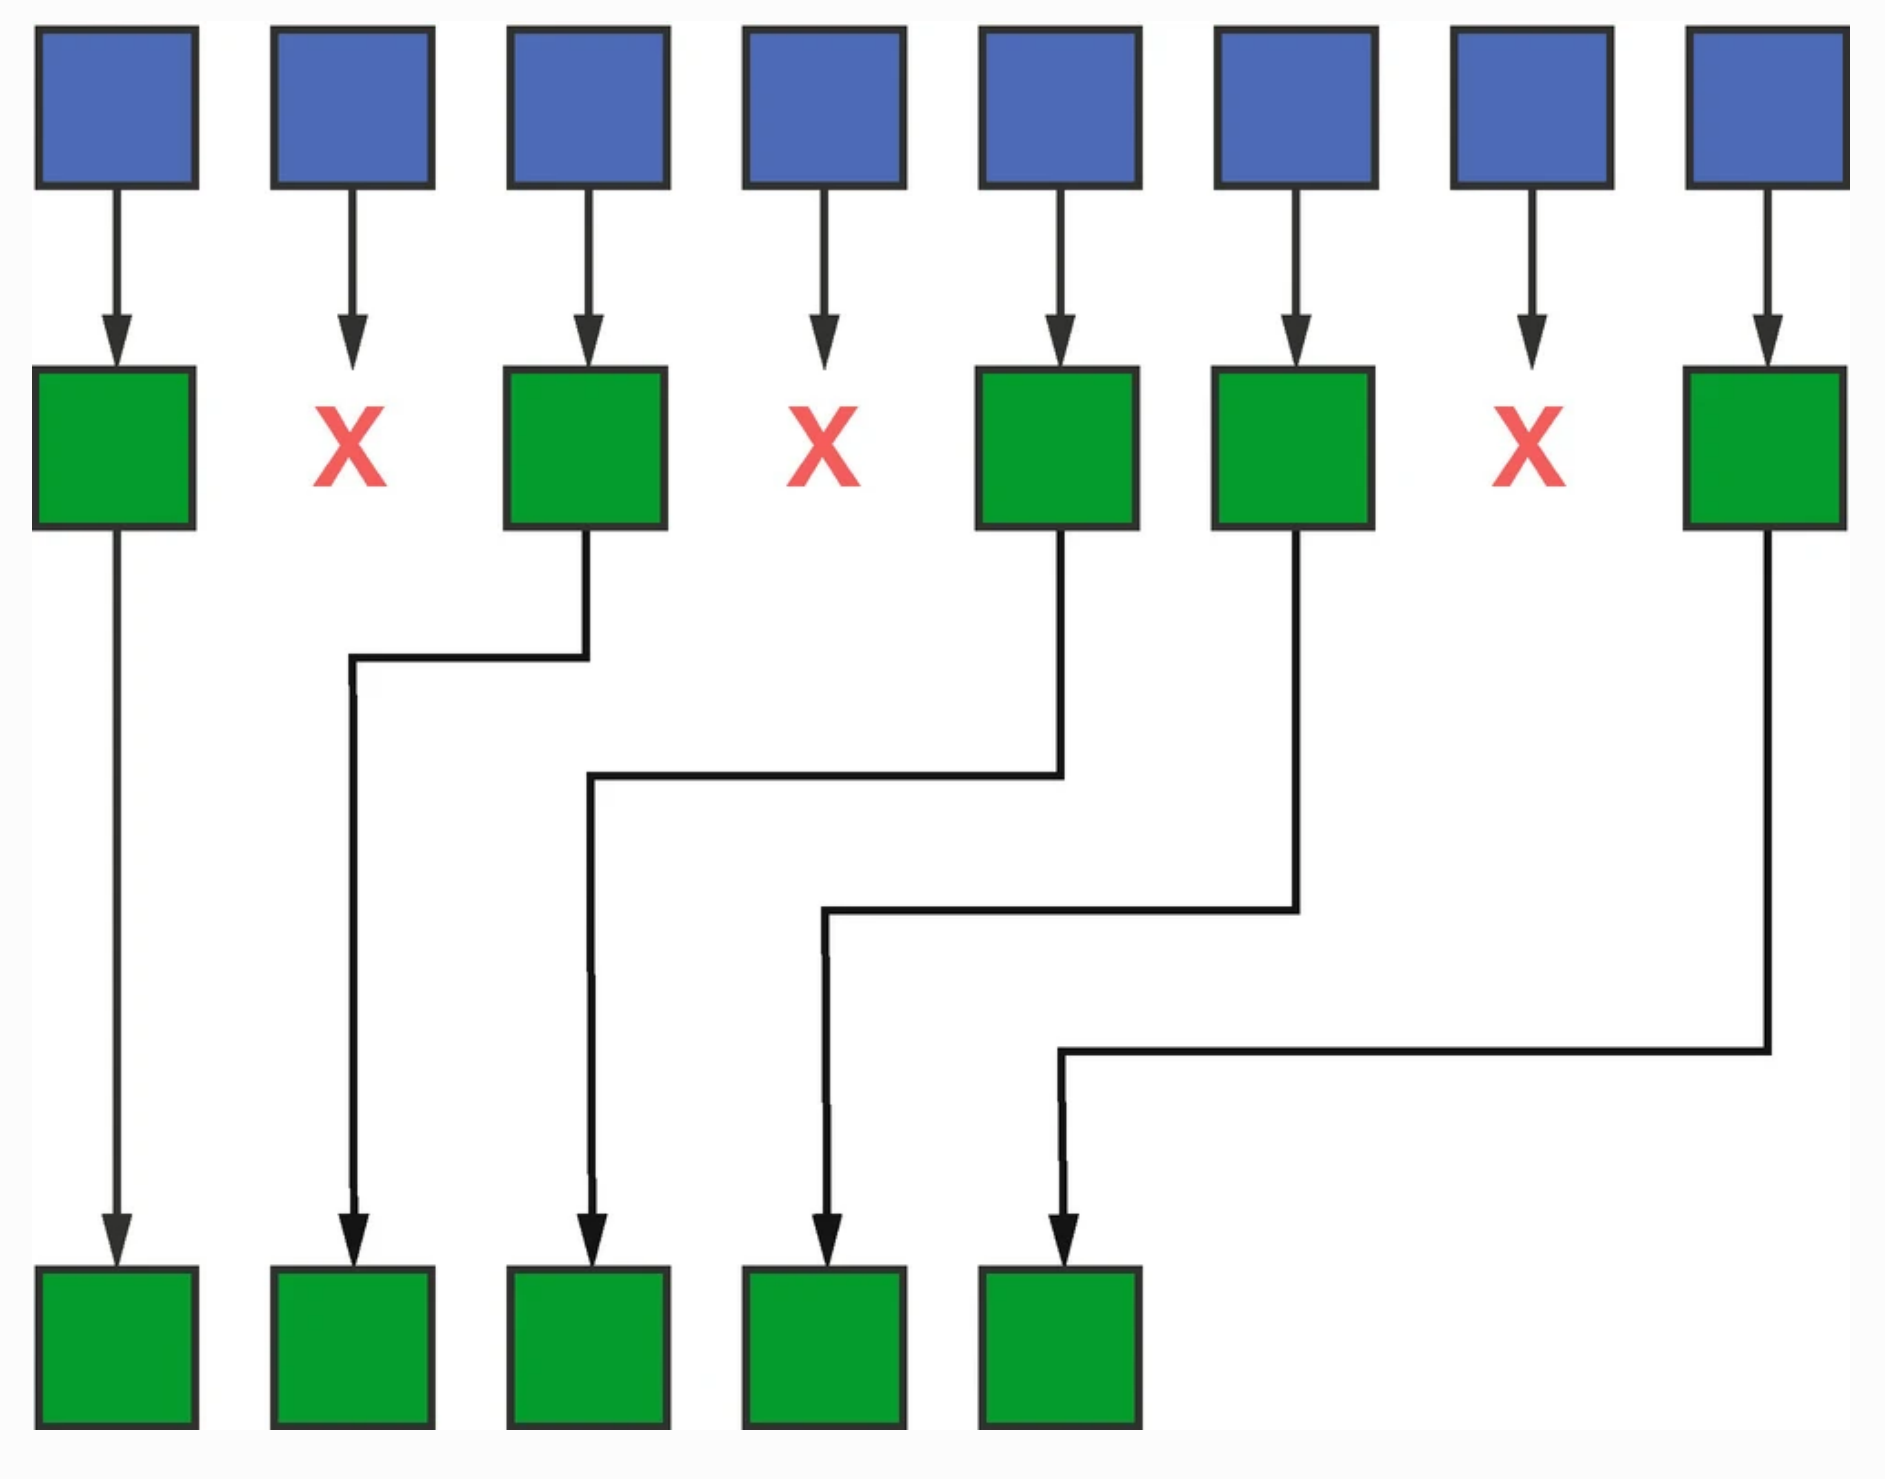
\includegraphics[scale=0.13]{Pack.png}
    \caption{https://link.springer.com/chapter/10.1007/978-1-4842-5574-2\_14/figures/6}
\end{figure}

\noindent We can do the pack in three steps:

\begin{enumerate}
  \item Compute a bit vector \texttt{bitVec}, where \texttt{bitVec[i]}=1\(\iff\) f(\texttt{arr[i]})=1. That is, an entry of the bit vector is 1 if the corresponding element fulfills the condition and 0 otherwise. This is a simple map that can be computed in one pass using the fork/join framework with a \(\mathcal{O}(log(n))\) span.
  \item Now we need to find the position in the final array of each element. To do so, we compute a prefix sum \texttt{bitSum} on the bit vector. Then, \texttt{bitSum[i]} tells us how many elements in \texttt{arr[0],...,arr[i]} fulfill the condition. In the previous section we saw how we can parallelize prefix-sum to have an \(\mathcal{O}(log(n))\) span as well.
  \item Using the information of the second step, we can compute the place of an element in the output array in the following way:
    \begin{minted}[]{java}
    if (bitVec[i] == 1) {
        res[bitSum[i]-1] = arr[i];
    }
    \end{minted}
    This is again a map, which we can also implement with \(\mathcal{O}(log(n))\) span.
\end{enumerate}

\noindent Since all of the steps have span \(\mathcal{O}(log(n))\), we can implement this parallel pack algorithm in \(\mathcal{O}(log(n))\) span. Since 1. and 3. are simple maps and the code for 2. is given in the previous section, we omit the Java implementation here.

\subsubsection{Case Study: Parallelizing QuickSort}
Having learned to parallelize multiple patterns, we try to apply some of them to parallelize a familiar algorithm: QuickSort. First, we remember that sequential QuickSort is an in-place algorithm that runs in \(\mathcal{O}(n*log(n))\) with the following steps:

\begin{enumerate}
  \item Pick a pivot element: \(\mathcal{O}(1)\)
  \item Partition the data (less than pivot, pivot, greater than pivot): \(\mathcal{O}(n)\)
  \item Recursively sort left and right part: \(2*T\left(\frac{n}{2}\right)\).
\end{enumerate}

\noindent We can trivially parallelize the recursive left and right sort using the fork/join framework. However, since partitioning the data is in \(\mathcal{O}(n)\), we cannot get a span better than \(\mathcal{O}(n)\). In order to improve this bound, we need to parallelize the data partitioning part.

To do so, let us think about what we really need to do to partition the array. All elements less than the pivot need to be selected and put to the \textit{left} in the array, while all elements greater than the pivot need to be selected and put to the \textit{right} in the array. However, if we allow this to not be performed in-place, this can be achieved with two packs: We pack all elements less than the pivot into a new array and all elements greater than the pivot into another new array. Then, we can combine those back into the original array and put the pivot element between them. Thanks to our parallel pack algorithm, this means \(\mathcal{O}(log(n))\) span to partition the array with \(\mathcal{O}(n)\) additional memory because the packs are not in-place.

Our recursion equation becomes \(T(n)=\mathcal{O}(log(n))+T\left(\frac{n}{2}\right)=\mathcal{O}((log(n))^{2}\), a great asymptotic improvement over the sequential \(\mathcal{O}(n*log(n))\).

We see that a repertoire of some basic parallel patterns helps us effectively parallelize more complex algorithms. Implementing this parallel QuickSort in Java is more involved (remember that we had to code around 80 lines for parallel prefix-sum, which is just a part of the parallel pack, which in turn is just a part of parallel QuickSort) and it is enough for us to realize how it could be done, since parallelizing algorithms in Java is not the main focus of the course.

\subsubsection{Parallelizing Algorithms on Different Datastructures}
So far, we always assumed arrays as our datastructure. What is so special about arrays though? It is their property of being able to access each element in \(\mathcal{O}(1)\).

\subsubsubsection{Span of Divide-And-Conquer Algorithms}
Let us recall what made parallel divide-and-conquer so effective. It was that we could reduce the span from \(\mathcal{O}(n)\) to \(\mathcal{O}\left(log(n)\right)\), which is the \textit{depth} of the task graph. Consider a critical path in this divide-and-conquer task graph (remember it looks like a binary tree). We make three observations:

\begin{itemize}
  \item There are \(\mathcal{O}\left(log(n)\right)\) vertices on the path (this is the depth of the task graph).
  \item The last vertex on the path is the computation of the base case. Let us say this takes \(\mathcal{O}(X)\) as it depends on the operation we want to compute.
  \item All other vertices on the path correspond to dividing up the data on subtasks and then combining the results. Time required to divide the work depends on the datastructure, so let us say it takes \(\mathcal{O}(Y(n))\). Let us also say that combining results takes \(\mathcal{O}(Z(n))\).
\end{itemize}

\noindent The time it takes to compute this critical path is thus \(\mathcal{O}\left(log(n)*(Y(n) + Z(n))\ +\ X\right)\), because we have to divide up the data \(log(n)\) times in \(\mathcal{O}(Y(n))\) each, compute the base case once in \(\mathcal{O}(X)\) and recombine results in \(\mathcal{O}(Z(n))\) \(log(n)\) times. The time it takes to compute the critical path is by definition the span, so this is also the span of a divide-and-conquer algorithm. Note however that the O-notation means it is an upper bound. In this case, the bound is not tight and depending on the functions X, Y and Z, we can get a better bound than the one suggested above.

Since for arrays, dividing up the work is possible in \(\mathcal{O}(1)\), that is, \(Y\equiv 1\), the span of divide-and-conquer algorithms (on arrays) is \(\mathcal{O}(log(n))\) for all operations, for which the base case (X) and recombining results (Z) is in \(\mathcal{O}(1)\). That is the case in particular for reductions and maps.

\subsubsubsection{Linked Lists}
For linked lists, accessing an element takes \(\mathcal{O}(n)\). Imagine we would want to sum all elements of a linked list using a divide-and-conquer approach. In order to divide the list in half, a subtask would have to traverse to the second half of the assigned chunk, which takes \(\mathcal{O}(n)\). Hence, \(Y\equiv n\) and thus we cannot get a span less than \(\mathcal{O}(n*log(n))\) using divide-and-conquer on linked lists. Divide-and-conquer does not make sense on a linked list due to the linear traversal time and we would be better of simply using a naive approach, where can at least get to \(\mathcal{O}(n)\).

Not all is bad though. Consider a long computation that takes \(\mathcal{O}(X)\), which we want to compute for each element of the linked list. Sequentially, this takes \(\mathcal{O}(n*X)\). The parallel span is \(\mathcal{O}(n + X)\) though. The critical path here is the task that needs to traverse to the last element of the list (\(\mathcal{O}(n)\)) and then compute the function (\(\mathcal{O}(X)\)).

\subsubsubsection{Balanced Trees}
Divide-and-conquer parallelism works well in balanced trees. Imagine we want to sum all elements in the tree. Dividing up the work can be done by forking the left and right child to process in parallel. Dividing up the work hence takes \(\mathcal{O}(1)\) and we get \(\mathcal{O}(h)\) span, where h is the height of the tree. In balanced trees, this is logarithmic in n.

\end{document}
